\documentclass[printmode,oneside,pl,eng]{mgr}  % do publikacji elektronicznej
% \documentclass[printmode,pl, eng]{mgr}  % do wydruku dwustronnego
%\documentclass[printmode,pl,draft]{mgr}  % do wydruku dwustronnego w~wersji roboczej
%\documentclass[printmode,en]{mgr}  % do wydruku dwustronnego ze stroną tytułową w~wersji angielskiej

%----------------------| Wybór strony kodowej |------------------------

\usepackage[utf8]{inputenc}

%-------------------------| Wybór kroju pisma |------------------------

%% Najpierw (chyba) należy wybrać czcionkę tekstu, potem matematyki

%% wybór czcionki Computer Concrete specjalnie zaprojektowanej do użycia 
%% z~czcionką matematyczną euler (nie ma ona niestety wersji bold - proponuje się więc użycie bolda z kroju
%%   Computer Modern Sans Serif)
%\usepackage{beton}             % ZALECANA DO SKŁADU TEKSTÓW PO ANGIELSKU
%\renewcommand{\bfdefault}{sbc} % to use Computer Modern Sans Serif demibold condensed fonts as bold 
%% choć może komuś bardziej podobać się będzie ten krój normalnej szerokości 
%\renewcommand{\bfdefault}{sb} % to use Computer Modern Sans Serif demibold fonts as bold 

%% alternatywny wybór Antykwy Półtawskiego - czcionki zaprojektowanej
%% specjalnie dla języka polskiego uwzględniającej jego rytm 
%\usepackage{antpolt}
%% alternatywny wybór Antykwy Toruńskiej - bardziej "współczesnej",
%% całkowicie polskiej czcionki
\usepackage{anttor}             % ZALECANA DO SKŁADU TEKSTÓW PO POLSKU
%\usepackage[math]{anttor}      % math włącza antykwę także w~matematyce
                                % ale chyba coś psuje :( (np. brak strzałek)

%% alternatywnie wybór czcionki URW Palladio
%\usepackage{newpxtext}  % Palatino font
%\linespread{1.05}  % Palatino needs more leading space (between lines)

%% ustawienie czcionki eulerowskiej do składu wyrażeń matematycznych
%\usepackage[euler-digits,small]{eulervm}
\usepackage{eulervm}

%% ustawienie czcionki bezszeryfowej Monospace (typewriter, code) font (last) - skład poleceń, wydruków programów
\usepackage[varqu,varl]{inconsolata}

%-------------------------| Sprawy polskie |------------------------

\usepackage[T1]{fontenc} % bez tego są złe znaki / { } w czcionce tt
                         % ale musi być użyty pakiet polski bez opcji
                         % wybierającej układ - gdy zamarkowane
                         % używamy pakiet polski z~opcją wyboru układu
\usepackage{polski}
%\usepackage[OT4]{polski} % domyślnie?

%---------------------------| Pakietologia |-------------------------

\usepackage{geometry}           % manipulowanie geometrią łamu
\usepackage{indentfirst}        % wcięcia akapitowe w pierwszych paragrafach rozdziałów
\usepackage[dvipsnames]{xcolor} % by mieć nazwy kolorów w~rodzaju \green
\usepackage{siunitx}
\usepackage{units}


%% zmiana formatowania tytulariów
%\usepackage[raggedleft]{titlesec}

\usepackage[titles]{tocloft}    % do formatowania spisów

%% modyfikacja odstępów między pozycjami w spisie treści
%% w razie potrzeby zmieniamy nieco odstępy przed rozdziałami i podrozdziałami w spisie
%% treści by uniknąć pojedynczego samotnego tytułu rozdziału/podrozdziału na dole/górze strony
%% i by ładnie się zmieściła notka o latechu
\addtolength{\cftbeforechapskip}{-1.3ex}
\addtolength{\cftbeforesecskip}{0.02ex}
 
%% %%% Bibliography %%%%%%%%%%%%%%%%%%%%%%%%%%%%%%%%%%%%%%%%%%%%%%%%%%%%%%%%%%%%%%%
%% \usepackage{xpatch}  % ?recommended for biblatex?
%% \usepackage[% biblatex has more styles, etc. than the default natbib
%%     backend=bibtex,  % by default it's biber,
%%                      % they say that biber is better but it didn't work for me
%%     citestyle=numeric-comp,  % cite by number, will collapse ranges, e.g. [3-6]
%%     bibstyle=numeric,  % printbibliography will show as [1], [2], ...
%%     giveninits=true  % use given/first names initials only, e.g. "K. Tchoń"
%% ]{biblatex}
%% % names bibtex, biber, biblatex and natbib are quite confusing, see:
%% % https://tex.stackexchange.com/questions/25701/bibtex-vs-biber-and-biblatex-vs-natbib


%%modyfikacja odstępów między pozycjami w bibliografii
\let\oldbibliography\thebibliography
\renewcommand{\thebibliography}[1]{%
  \oldbibliography{#1}%
  \setlength{\itemsep}{0pt plus 0.3ex}%
}

%% ustawienie maksymalnej liczby i obszaru dla obiektów pływających (rysunków, tabel)
\setcounter{topnumber}{3}
\setcounter{totalnumber}{4}
\renewcommand{\topfraction}{.8}

\usepackage{graphicx}                % dołaczanie i manipulowanie grafikami
\usepackage[export]{adjustbox}       % więcej komend operujących na "pudełkach"
\usepackage[caption = false]{subfig} % obsługa rysunków z częściami

%\usepackage{svg}                % dołączanie grafik w formacie svg
%\usepackage[inkscapepath=svgdir]{svg}  % w nowszych wersjach

\usepackage{tikz}               % dołączanie grafik w formacie TikZ
\usepackage{tikz-timing}
\usepackage{tikz-3dplot}
\usepackage{makecell}           % trochę tikzowej magii
    \tikzstyle{block} = [draw, fill=blue!20, rectangle, 
     minimum height=3em, minimum width=6em]
    \tikzstyle{sum} = [draw, fill=blue!20, circle, node distance=3.5cm]
    \tikzstyle{input} = [coordinate]
    \tikzstyle{output} = [coordinate]
    \tikzstyle{pinstyle} = [pin edge={to-,thin,black}]    
    \usetikzlibrary{arrows,automata,calc,positioning}
\usepackage{standalone}  

\usepackage{pgfplots}           % do robienia wykresów 
\pgfplotsset{compat=1.5}        %% why 1.5? pl. update

\usepackage{mathtools}          % doskonałe pakiety rozszerzające do matematyki
\usepackage{amssymb, amsfonts}  % mathtools zastępuje amsmath (naprawione błedy, dodane rozszerzenia) 
\usepackage{wasysym}            % trochę więcej różnych symboli (buźki)
%\usepackage[fleqn]{mathtools}  % równania w wersji dosuniętej w lewo
%% automatyczne numerowanie jedynie tych równań, do których są odwołania w~tekście
%\mathtoolsset{showonlyrefs=true}

%% symbole do oznaczania stopek w~miejsce liczb
\renewcommand{\thefootnote}{\fnsymbol{footnote}}
%% powtórzone z latex.ltx - w przeciwnym razie znika symbol \textbardbl przy
%% wybranej Antykwie Toruńskiej (sprawdzić co z innymi definicjami z omsenc.def,
%% sprawdzić czy też przy innych czcionkach)
\DeclareTextSymbolDefault{\textbardbl}{OMS}
%% automatyczne resetowanie wartości licznika stopek użyteczne przy użyciu symboli
%% do oznaczania stopek w~miejsce liczb (liczba dostępnych symboli wynosi tylko 9)
\usepackage{etoolbox,pdftexcmds}
\makeatletter
\patchcmd{\footnote}
  {\stepcounter\@mpfn}
%  {\stepcounter\@mpfn\check@overflow\@mpfn} %%było w~przykładzie
  {\stepcounter\@mpfn\check@overflow}
  {}{}
\newcommand{\check@overflow}{%
  \ifnum\pdf@strcmp{\@mpfn}{footnote}=\z@
    \ifnum\value{footnote}>9  %
      \setcounter{footnote}{1}%
    \fi
  \fi
}
\makeatother

\usepackage{hyperref}           % obsługa aktywnych odnośników i hypertekstu
\usepackage{url}                % obsługa adresów url

%% pakiet minted do wydruków programów
%% 'minted' gives much better highlight then the default listings,
%% but it reqires Python with Pygments (check the documentation of minted)
%% it also requires passing '-shell-escape' option to pdflatex during compilation
\usepackage[%
  cache=false,
  chapter,
  %    outputdir=build,  % if building in separate directory, this must be included
                         % ale nie zawsze działa poprawnie :( 
    newfloat  % required if multi-page floating listings are needed (see below)
]{minted}  % (note: from my experience must be loaded before 'csquotes')
%% by wybrać inny styl - lista dostępnych styli: pygmentize -L styles
%\usemintedstyle{igor}
\SetupFloatingEnvironment{listing}{name=Wydruk}
%% kolor tła używany w~wydrukach
\definecolor{OurListingBackground}{rgb}{0.95,0.95,0.95}
%% fix the minted@colorbg environment bug
\makeatletter
\renewenvironment{minted@colorbg}[1]
 {\def\minted@bgcol{#1}%
  \noindent
  \begin{lrbox}{\minted@bgbox}
  \begin{minipage}{\linewidth-2\fboxsep}}
 {\end{minipage}%
  \end{lrbox}%
  \setlength{\topsep}{\bigskipamount}% set the vertical space
  \trivlist\item\relax % ensure going to a new line
  \colorbox{\minted@bgcol}{\usebox{\minted@bgbox}}%
  \endtrivlist % close the trivlist
 }
\makeatother
%% koniec ustawień pakietu minted

%\usepackage{csquotes}

%%pakiet do robienia notatek w trakcie pracy
\usepackage[textsize=footnotesize]{todonotes}
\makeatletter   %spolszczenie
\renewcommand{\@todonotes@todolistname}{Do zrobienia}
\renewcommand{\@todonotes@MissingFigureText}{Rysunek}
\renewcommand{\@todonotes@MissingFigureUp}{{\small Brakujący}}
\renewcommand{\@todonotes@MissingFigureDown}{{\small rysunek}}
\makeatother

%% dodaje w pliku wynikowym klucze etykiet i referencji - wygodne przy pracy nad tekstem
%\usepackage{showkeys}

\newcommand*{\captionsource}[2]{%
  \caption[{#1}]{%
    #1%
    . Źródło: #2%
  }%
}

%%inne przydatne
%\usepackage{fancyhdr}
%\usepackage{fancyvrb}
%\usepackage{lipsum}  
%\usepackage{listings}  %% alternatywa do używanego tutaj pakietu minted 

%-----------------------| End of pakietologia |----------------------

%---------------------------| Tytularia |---------------------------

% Zmień dane stosownie do tytułu i autora pracy tutaj
% ALE TEŻ I W POLECENIU \pdftitle NIECO PONIŻEJ! (Hyper data general configuration)
\author{Krystian Mirek}
\title{Wieloodbiornikowy czujnik ultradźwiękowy z mikrofonami MEMS}
\engtitle{Top is a top. Case study}
\supervisor{Dr inż. Bogdan Kreczmer,\\ Katedra Cybernetyki i~Robotyki}
\field{Automatyka i~Robotyka (AIR)}
\specialisation{Robotyka (ARR)}
\date{2023}

%-------------------------| Hyper data general configuration |------------------------

\hypersetup{unicode,
                          % DANE DOKUMENTACJI
   pdfauthor={Krystian Mirek},
   pdftitle={Wieloodbiornikowy czujnik ultradźwiękowy z mikrofonami MEMS},
   pdfsubject={Praca dyplomowa inżynierska - przykład i~wytyczne},
   pdfkeywords={bąk, Lagrange top, Euler top, praca dyplomowa, formatowanie, wytyczne},
                          % USTAWIENIA DOKUMENTU
   pdfpagemode=UseOutlines,   % otwiera dokument w trybie jednej strony
   pdfpagelayout=SinglePage,  %
   pdfstartview={Fit},        %
   pdfstartpage=1,            % na podanej stronie
   bookmarksopen=true,        % rozwinięcie zakładek
   bookmarksopenlevel=1,      % do jakiego poziomu
   colorlinks=true,       % kolorowanie odnośników zamiast ramki wokół nich
   breaklinks,            %
   citecolor=cyan,        % kolor odnośników do bibliografii, domyślnie zielony
   filecolor=red,         % kolor odnośników do lokalnych plików, domyśnie magenta
   linkcolor=blue,        % kolor odnośników wewnętrznych, domyślnie czerwony
   menucolor=green,       % kolor pozycji menu Acrobata, domyślnie czerwony
   urlcolor=blue          % kolor odnośników do adresów internetowych, domyślnie cyan
}

%-------------------------| Geometria strony |-----------------------------

\geometry{
    top = 25mm,
    headheight = 15mm,
    headsep = 3mm,
    textheight = 24cm,
    textwidth = 16cm,
    marginparwidth = 25mm
}

%---------------------| Często używane polecenia |-------------------

\newcommand{\red}{\color{red}}
\def\BibTeX{{\rm B\kern-.05em{\sc i\kern-.025em b}\kern-.08em
    T\kern-.1667em\lower.7ex\hbox{E}\kern-.125emX}}

\newtheorem{uwaga}{Uwaga}
\newtheorem{twr}{Twierdzenie}
%------------------------------------| END |-------------------------------------

%----------------------------| Definicje symboli matematycznych |-------------------------

\newcommand{\angmom}{\boldsymbol{m}}
\newcommand{\bdvelo}{\boldsymbol{\omega}_B}
\newcommand{\grav}{\boldsymbol{g}}
\newcommand{\lagran}{L(\boldsymbol{q},\boldsymbol{\dot{q}})}
\newcommand{\COMvec}{\boldsymbol{r}_B}
\newcommand{\ee}{\boldsymbol{e}}
\newcommand{\FF}{\boldsymbol{F}}
\newcommand{\xx}{\boldsymbol{x}}
\newcommand{\qq}{\boldsymbol{q}}
\newcommand{\RR}{\boldsymbol{R}}
\newcommand{\TT}{\boldsymbol{T}}
\newcommand{\pp}{\boldsymbol{p}}
\newcommand{\iner}{\boldsymbol{I}_B}
\newcommand{\vv}{\boldsymbol{v}}
\newcommand{\bbs}{\boldsymbol}
\DeclareMathOperator{\const}{const}
\DeclareMathOperator*{\rank}{rank}  %star changes sub- and superscripts placement
%------------------------------------| END |-------------------------------------

%--------------------------| Ścieżki do rysunków |-------------------------------

\graphicspath{{./figures/chapter_01/}{./figures/chapter_02/}{./figures/chapter_03/}{./figures/chapter_04/}{./figures/chapter_05/}{./figures/chapter_06/}{./figures/chapter_07/}{./figures/chapter_08/}{./figures/chapter_09/}}

%--------| kontrola dołączanych plików - wygodne przy pracy nad tekstem |--------

%\includeonly{sources/Od_Autora,sources/02_czym_jest_bak}

%-------------------------| The document starts here |-------------------------------
\begin{document}

\pdfbookmark{Strona tytułowa}{tytul}
\maketitle

\section*{Streszczenie}\label{chapter:streszczenie}
Celem pracy jest budowa sonaru będącego czujnikiem ultradźwiękowym z mikrofonami MEMS. 
Urządzenie to ma posłużyć do wyznaczania kąta azymutu oraz elewacji badanego obiektu.
Zakres prac sprzętowych obejmuje projekt i wykonanie układów elektronicznych oraz obudowy urządzenia. 
Część oprogramowania wymaga opracowania programu mikrokontrolera odpowiadającego za sterowanie przetwornikami, przechwytywanie sygnałów oraz komunikację z komputerem.

Pracę podzielono na rozdziały przedstawiające następujące zagadnienia. W rozdziale drugim opisany został cel projektu oraz wymagania stawiane wobec urządzenia. 
Trzeci rozdział przedstawia proces doboru odbiorników sygnału, które są najważniejszym elementem konstrukcji. 
W czwartym pochylono się nad analizą najistotniejszych problemów występujących w tego typu sonarach. Rozdział piąty opisuje specyfikację pracy z urządzeniem wod strony użytkownika.
W rozdziale szóstym dogłębnie został przedstawiony proces projektowania układów elektronicznych oraz oprogramowania. Siódmy rozdział przedstawia realizację w postaci wizualizacji oraz opisu wykonanego urządzenia.
Przedostatni rozdział ma na celu zobrazowanie metodologii badawczej oraz efektów działania składowych elementów całego systemu. Rozdział ostatni podsumowuje pracę dyplomową.

Cel pracy został osiągnięty częściowo. Urządzenie zostało wykonane i wszystkie jego elementy przetestowane. Sprzętowa część spełnia wszystkie cele, 
lecz w obecnym systemie oprogramowania, pomimo spełnienia warunków komunikacji z użytkownikiem, nie udało się dokonać zapisu danych.

\textbf{Słowa kluczowe: }sonar, ultradźwięki, przetwornik, czujnik, systemy wbudowane, elektronika, filtr, wzmacniacz, mikrokontroler


\section*{Abstract}\label{chapter:abstract}
Goal of thesis is to make sonar device as ultrasonic sensor with MEMS microphones.
Device is going to be used to estimate angle of azimuth and elevation of tested object.
Scope of hardware work includes designing and manufacturing electronics and housing of the device. 
Software part includes developing program responsible for control of the transducers, capturing signals and communication with PC.

Thesis is divided by chapter that explains the following issues. Second chapter shows goals and assumptions of whole project. 
Third chapter explains process behind choosing the right sensor. 
Fourth chapter analyses problems that encounters in designing sonars.
Fifth chapter describes user requirements.
Sixth chapter shows process of designing hardware and software.
Seventh chapter describes implementation in form of photos and description.
Eight chapter shows test methodology and effects of working device.
Last chapter is the summary of whole thesis.

Goal of work is accomplished partly. Device has been made and all of its components were tested. 
Hardware part meets all of the expectations but in current software architecture it is impossible to save captured data fast enough.

\textbf{Keywords: }sonar, ultrasonic, transducer, sensor, embedded system, electronics, filter, amplifier, microcontroller 
%% informacja o sposobie udostępniania tego dokumentu
% \thispagestyle{empty}
\mbox{}
\vfill

\noindent
{\bf Robert Muszyński, Roberto Orozco}\\
{\bf Wrocław 2022}\\[2ex]
  
\includegraphics[width=0.18\textwidth]{figures/CC-BY-SA_icon_svg.png}\hfill
\begin{minipage}[b]{0.79\textwidth}
 \small Szablon jest dostępny na licencji Creative Commons: \emph{Uznanie au\-tor\-stwa-Na tych samych warunkach 4.0 Polska}
\end{minipage}\vspace{2ex}

\noindent
{\normalsize Utwór udostępniany na licencji Creative Commons: uznanie
  autorstwa, na tych samych warunkach. Udziela się zezwolenia do
  kopiowania, rozpowszechniania i/lub modyfikacji treści utworu
  zgodnie z zasadami w/w licencji opublikowanej przez Creative
  Commons. Licencja wymaga podania oryginalnego autora utworu, a
  dystrybucja materiałów pochodnych może odbywać się tylko na tych
  samych warunkach (nie można zastrzec, w jakikolwiek sposób
  ograniczyć, ani rozszerzyć praw do nich). Tekst licencji jest
  dostępny pod
  adresem: \url{https://creativecommons.org/licenses/by-sa/4.0/legalcode.pl}. Podczas
  redakcji pracy dyplomowej notkę tę można usunąć, licencja dotyczy
  bowiem zredagowanego opisu, a nie samego latechowego
  szablonu.  Szablon można wykorzystywać bez wzmiankowania o
  jego autorze.}


%% dedykacja
%%\dedication{6cm}{To jest przykładowa treść opcjonalnej dedykacji,
%%  należy ją zmienić lub usunąć w całości polecenie
%%  \texttt{\textbackslash dedication}}

\cleardoublepage
\pdfbookmark{\contentsname}{Contents}
\tableofcontents            %spis treści
\markboth{\contentsname}{\contentsname}
%%\newpage
%\thispagestyle{empty}
%\cleardoublepage
%\thispagestyle{plain}

\mbox{}\vfill\hfill
\begin{minipage}{0.5\linewidth} 
  {\tiny \noindent Do składu pracy wykorzystano system przygotowania
    dokumentów~\LaTeX, opracowany przez
    L.~Lamporta\index{latex>\LaTeX} [Lam94], będący nakładką
    systemu \TeX, [Knu86a,Knu86b].  Matematyczne czcionki o nazwie
    {AMS Euler}, których używamy w tej pracy, zostały przygotowane
    przez H.\ Zapfa [KZ86], przy współpracy z~D.\ Knuthem i~jego
    studentami, na zlecenie Amerykańskiego Towarzystwa Matematycznego.
    %% Przy wybranej Antykwie Toruńskiej/Półtawskiego odznacz odpowiednio poniższe
    Wybrane czcionki składu tekstu, Antykwa Toruńska [Now97] -- jeden
    %Wybrane czcionki składu tekstu, Antykwa Półtawskiego [Now99] -- jeden
    z~nielicznych krojów pisma zaprojektowany specjalnie dla języka
    polskiego w~sposób uwzględniający jego rytm -- w~odczuciu autora
    doskonale współgrają z~kształtem czcionki {AMS Euler}, pozwalając
    na uzyskanie harmonijnej całości.
    % %% Przy wybranych czcionkach Concrete odznacz poniższe
    % Czcionki składu tekstu, zwane {Concrete Roman} i {Concrete
    %   Italic}, należące do knuthowskiej rodziny czcionek {Computer
    %   Modern}, zostały specjalnie przystosowane do kształtu czcionki
    % {AMS Euler} na potrzeby książki [GKP96].
    % %% Przy wybranych czcionkach URW Palladio odznacz poniższe
    % Czcionka składu tekstu, zwana URW Palladio jest klonem zapfoskiej rodziny
    % czcionek o~nazwie Palatino [LPn05] i~zdaniem autora świetnie współgra
    % z~kształtem czcionki {AMS Euler}.
    Składu bezszeryfowego tekstu maszynowego dokonano z~użyciem
    opracowanej przez R. Leviena czcionki o~nazwie Inconsolata
    [Lev15]\footnote{\red\tiny Chyba warto takie informacje szerzyć}.


\vspace{-4mm}

 \makeatletter
\renewenvironment{thebibliography}[1]
     {%
        \tiny%
      \list{\@biblabel{\@arabic\c@enumiv}}%
           {\settowidth\labelwidth{\@biblabel{#1}}%
\setlength{\itemsep}{2.5mm}
            \leftmargin\labelwidth
            \advance\leftmargin\labelsep
            \@openbib@code
            \usecounter{enumiv}%
            \let\p@enumiv\@empty
            \renewcommand\theenumiv{\@arabic\c@enumiv}}%
      \sloppy\clubpenalty4000\widowpenalty4000%
      \sfcode`\.\@m\vspace{5mm}}
     {\def\@noitemerr
       {\@latex@warning{Empty `thebibliography' environment}}%
      \endlist}

\makeatother

\begin{thebibliography}{Knu86b}

% %% Odmarkować pozycję gdy wybrane czcionki Concrete
% \bibitem[GKP96]{GKP96loc}
% R.~L. Graham, D.~E. Knuth i O.~Patashnik,
% \newblock { Matematyka konkretna}.
% \newblock PWN, Warszawa, 1996.\vspace{-3mm}

\bibitem[Knu86a]{Knuth86loc}
D.~E. Knuth,
\newblock { The \TeX book, volume {A} of Computers and Typesetting}.
\newblock Addison-Wesley, Reading, 1986.\vspace{-3mm}

\bibitem[Knu86b]{Knuth86aloc}
D.~E. Knuth,
\newblock { \TeX: {The} Program, volume {B} of Computers and Typesetting}.
\newblock Addison-Wesley, Reading, 1986.\vspace{-3mm}

\bibitem[KZ86]{KnZa89loc}
D.~E. Knuth i H.~Zapf,
\newblock {AMS} {Euler} --- {A} new typeface for mathematics.
\newblock { Scholary Publishing}, {20}:131--157, 1986.\vspace{-3mm}

\bibitem[Lam94]{Lamport94loc}
L.~Lamport,
\newblock { \LaTeX: A Document Preparation System}.
\newblock Addison-\mbox{-Wesley}, Reading, 1994.\vspace{-3mm}

\bibitem[Lev15]{Levien15loc}
R.~Levien,
\newblock {Inconsolata}.
\newblock \url{https://levien.com/type/myfonts/inconsolata.html}, 2015.\vspace{-3mm}

% %% Odmarkować pozycję przy wybranej czcionce URW Palladio
% \bibitem[LPn05]{LinotypePalatino05loc}
% Linotype Palatino nova: A classical typeface redesigned by Hermann Zapf,
% \newblock Linotype Library GmbH, 2005.\vspace{-2mm}

%% Odmarkować pozycję przy wybranej Antykwie Toruńskiej
\bibitem[Now97]{nowacki97loc}
J.~Nowacki,
\newblock {Antykwa} {Toruńska} -– od początku do końca polska czcionka.
\newblock {\em Biuletyn Polskiej Grupy Użytkowników Systemu \TeX}, 9:26--27,
  \nolinebreak1997.\vspace{-2mm}

% %% Odmarkować pozycję przy wybranej Antykwie Półtawskiego
% \bibitem[Now99]{nowacki99}
% J.~Nowacki,
% \newblock Piórkiem i {MetaPost-em}, czyli {Antykwa} {Półtawskiego}.
% \newblock {\em Biuletyn Polskiej Grupy Użytkowników Systemu \TeX}, 12:49--53,
%   \nolinebreak1999.\vspace{-2mm}

\end{thebibliography}
}
\end{minipage}
       %notka o systemie składu i czcionkach
%% Side note about LaTeX and the fonts being used in the thesis
\mbox{}\vfill\hfill
\begin{minipage}{0.618033988749895\textwidth}
    \begin{refsection}[font-note-literature.bib] % separate bibliography for this minipage
                                                 % this resource was added with \addsectionbib
        {% smaller font for paragraph and bibliography
            \scriptsize%
            \renewcommand*{\bibfont}{\scriptsize}%
            \noindent%
            %
            For typesetting this thesis,
            the~\LaTeX{} document preparation system has been used.
            \LaTeX{} has been developed by L.~Lamport~\cite{lamport:latex},
            and~is an~overlay on top of the~\TeX{} system~\cite{knuth:texbook}.
            %
            Mathematical fonts called AMS~Euler which have been used in~this document,
            have been commissioned by the American Mathematical Society
            and~designed by H.\ Zapf~\cite{zapf:ams-euler} with the assistance of D.\ Knuth and his students.
            %
            The~URW~Palladio font, used for roman text,
            is a~clone of H.\ Zapf's old-style typeface called Palatino~\cite{zapf:palatino}.
            %
            Typesetting of sans-serif monospaced text has been done using
            Inconsolata font, created by R.\ Levien~\cite{levien:inconsolata}.
            %
            \noindent
            \printbibliography[heading=none,locallabelwidth=true] % print section bibliography
        }
    \end{refsection}
\end{minipage}
   %przykładowa wersja angielska notki - używa pakietu biblatex

%---------------------------| Część właściwa dokumentu |---------------------------

%\chapter*{Od Autorów}
\addcontentsline{toc}{chapter}{Od Autorów}
\markboth{Od Autorów}{Od Autorów}

Niniejszy przykład przygotowano celem ułatwienia opracowania prac dyplomowych z~wykorzystaniem dostarczonego przez Adama Ratajczaka stylu \texttt{mgr} systemu \LaTeX{}. Styl \texttt{mgr} służy do przygotowywania prac dyplomowych na Wydziale Elektroniki, Fotoniki i~Mikrosystemów oraz Wydziale Informatyki i~Telekomunikacji Politechniki Wrocławskiej i~jego głównym zadaniem jest odpowiednie sformatowanie strony tytułowej dokumentu\footnote{W razie potrzeby plik z~opisem klasy \texttt{mgr} można znaleźć na stronie autora \cite{Ratajczak}; tam też można znaleźć dokument szczegółowo opisujący sposób korzystania z~klasy \texttt{mgr} (\texttt{manual.pdf}) -- prezentowany tu przykład zawiera już najnowszą wersję pliku ze stylem \texttt{mgr}.}. Aktualną wersję prezentowanego przykładu można znaleźć na stronie internetowej \cite{wzor_praca} w~części ,,Inne materiały''\footnote{Informacje o~zauważonych błędach/brakach prosimy kierować na adres \texttt{mucha@pwr.edu.pl}.}. Więcej porad technicznych dotyczących składu pracy dyplomowej można znaleźć w~szablonie przygotowanym przez Tomasza Kubika \cite{kubik}. Listę zmian pozwalających przekształcić ten przykładowy dokument w~swoją własną pracę dyplomową zebrano w~podrozdziale~\ref{sec:listakontrolna}.

Dostarczony zestaw plików zawiera docelowy plik wzorcowy dokumentu z~pracą dyplomową w~formacie PDF \texttt{praca\_dyplomowa\_wzor.pdf} (który pewnie właśnie czytasz) oraz archiwum \texttt{praca\_dyplomowa\_wzor.zip}\footnote{Po jego rozpakowaniu otrzymujemy katalog \texttt{praca\_dyplomowa\_wzor} z~wszystkimi niezbędnymi do pracy plikami -- w~tym katalogu przeprowadzamy opisaną poniżej kompilację. By edytować dokument w~systemie Overleaf wystarczy wczytać do niego nierozpakowane archiwum (\texttt{New Project} $\rightarrow$ \texttt{Upload Project}).} zawierające zestaw jego plików źródłowych: plik główny \texttt{main.tex}\footnote{Pliki źródłowe przygotowano z~zastosowaniem systemu kodowania znaków UTF8 i~windowsowymi znakami nowej linii (CRLF). Konwersja znaków nowej linii do formatu uniksowgo (zazwyczaj niepotrzebna): \texttt{dos2unix plik\_we plik\_wy} lub \texttt{tr -d '\textbackslash r' < plik\_we > plik\_wy}.}, pliki z~treścią rozdziałów (znajdujące się w~katalogu \texttt{sources}), pliki rysunków (katalog \texttt{figures}). By skompilować dostarczone źródła do postaci wynikowej należy użyć kompilatora \LaTeX{}a oraz \BibTeX{}a w~sekwencji\footnote{Zakładamy tu, że wykorzystywana jest lokalna instalacja \LaTeX{}a z~poziomu powłoki tekstowej (np. \texttt{bash}). Takie rozwiązanie pozwala na pracę bez dostępu do internetu, jest bardzo szybkie i~daje się łatwo ,,automatyzować'' wedle potrzeby -- przez użycie skryptów powłoki, uruchamianie procesu kompilacji z~poziomu używanego edytora (np. emacsa:), integrację z~lokalną ,,wyświetlarką pdfów''. Warto spróbować! Przy korzystaniu z~innych rozwiązań, jak te wymienione w~podrozdziale~\ref{narzedzia}, należy zadbać, by w~ich ramach została wykonana odpowiednia sekwencja poleceń w~celu uzyskania aktualnego, wynikowego pliku PDF.}\footnote{W~niektórych systemach może potrzebne być użycie opcji pdflatecha \texttt{--shell-escape}.}\vspace{-3mm}
\begin{verbatim}
  pdflatex main
  bibtex main
  pdflatex main
  pdflatex main
\end{verbatim}
Bezbłędny przebieg wykonania powyższych poleceń wyprodukuje plik \texttt{main.pdf}, który powinien wyglądać identycznie jak ten wzorzec, co równocześnie potwierdzi poprawność i~kompletność wykorzystywanej instancji systemu \LaTeX. Dokument można kompilować we fragmentach z~zachowaniem poprawności wszystkich odwołań używając w~jego preambule polecenie \texttt{\textbackslash includeonly} z~podaną listą plików rozdziałów do dołączenia\footnote{Przykład użycia zamieszczono w~pliku \texttt{main.tex}.}.

W~tym przykładzie zdecydowano się na wykorzystanie do składu tekstu kroju pisma zaprojektowanego specjalnie dla języka polskiego o~nazwie Antykwa Toruńska \cite{antykwa,antykwab} wraz matematyczną czcionką o~nazwie AMS Euler \cite{eulerfont}, o~czym napisano w~dodanej pod spisem treści notce. Domyślne kroje pisma można łatwo przywrócić usuwając odpowiednie pakiety z~preambuły dokumentu\footnote{W preambule pokazano także, w~jaki sposób można włączyć inne kroje -- zwracamy uwagę, szczególnie osób piszących prace po angielsku, na kroje o~nazwach Computer Concrete oraz URW Palladio (pierwszy będący odmianą kroju Concrete Roman, zaś drugi kroju Palatino) \cite{concr, palla, antyk}.}. 

Prezentowany dokument, oprócz wskazania sposobu wykorzystania stylu \texttt{mgr}, opisuje podstawowe zasady tworzenia pracy dyplomowej. Jednakże należy podkreślić, że intencją autorów nie jest dostarczenie jeszcze jednego dokumentu traktującego o~metodach formatowania tekstu w~środowisku \LaTeX, ale zilustrowanie w~jednym miejscu sposobów uzyskania podstawowych elementów występujących w~typowej pracy dyplomowej\footnote{Dziś częstokroć dany efekt można uzyskać w~\LaTeX{}u na kilka sposobów i~wybór/znalezienie tego ,,najlepszego/właściwego'' może zająć sporo czasu. Stąd pomysł, by w~tym dokumencie podzielić się ,,doświadczeniem'' zdobytym przez wcześniejsze ,,pokolenia dyplomantów''. Jeśli masz więc jakieś uwagi śmiało pisz na \texttt{mucha@pwr.edu.pl}.}. Zamysł całości jest taki: Znajdź w~dostarczonym pdfie element, którego potrzebujesz i~zobacz w~jego źródłach, w~jaki sposób został uzyskany.

W~kolejnych rozdziałach tekst zapisany kolorem czerwonym stanowi komentarz do przytoczonych fragmentów pracy autorstwa Roberto Orozco \cite{roberto}, zwracający uwagę na rzeczy, które te fragmenty ilustrują. Komentarz każdorazowo dotyczy tekstu go poprzedzającego. W~źródle dokumentu można zobaczyć jak dany efekt uzyskano. A~poniżej zebrano podstawowe wytyczne dotyczące redakcji tekstu. Więcej o~zasadach użycia systemu \LaTeX{} można poczytać w~,,Nie za krótkim wprowadzeniu\ldots'' \cite{lshort2e} oraz szerzej w~,,Książce kucharskiej\ldots'' \cite{latex_kucharska}. Łagodne wprowadzenie do \LaTeX{}a zapewnia także kurs w~pdfie \cite{lshortpie}, kurs w~htmlu \cite{latex_kurs}, czy dokumentacja środowiska Overleaf \cite{latex_overleaf}. W~razie czego warto też zajrzeć na stronę Wikibooks \cite{latex_wiki2}.

Autorzy są wdzięczni Jędrzejowi Boczarowi, dyplomantowi specjalności Embedded Robotics w~roku 2019, za uprzejmą współpracę i~recenzję całości \cite{jedrzej}.

\section{Narzędzia}
\label{narzedzia}

\begin{enumerate}
%\setlength{\itemsep}{0pt}
\item \LaTeX{} jest językiem znaczników do formatowania dokumentów tekstowych, także zawierających elementy graficzne, który dostarcza zestawu makr stanowiących nadbudowę dla systemu składu \TeX, \cite{latex, latex_wiki, latex_wiki2}. Podstawowym oprogramowaniem służącym do kompilacji dokumentów opisanych w~tym języku jest system \LaTeX\footnote{który korzystając z~systemu \TeX{} na podstawie plików źródłowych produkuje plik wynikowy w~formacie \texttt{DVI} (\emph{ang. device independent}) stanowiący bazę do uzyskania innych formatów jak PDF czy PS \cite{dvi_wiki}}. Jednakże ponieważ obecnie dostępnych jest kilka alternatywnych dla \TeX{}a narzędzi, takich jak pdf\TeX, Xe\TeX{} czy Lua\TeX, towarzyszą im dedykowane systemy kompilacji jak pdf\LaTeX{} czy Xe\LaTeX. Autorzy tego dokumentu do jego kompilacji wykorzystali system pdf\LaTeX\footnote{który na podstawie plików źródłowych produkuje bezpośrednio plik wynikowy w~formacie PDF}, zaś zainteresowanych ,,innymi smakami \TeX{}a'' odsyłają do takich pozycji jak \cite{latex_kucharska,tex_legacy,xxxtex}.
  
\item Ponieważ sam \LaTeX{} jest systemem składu tekstu wyposażonym jedynie w~interfejs wiersza poleceń (\emph{ang. command-line interface})\footnote{nazywany przez niektórych interfejsem linii komend}, do pracy z~nim potrzebny jest edytor tekstowy, który pozwoli wprowadzić pożądaną treść do komputera. Wygodnie jest korzystać w~tym celu z~któregoś z~edytorów dostosowanych do składni \LaTeX{}a\footnote{Ale oczywiście możliwe jest użycie dowolnego edytora tekstu, byle tylko pozwalał on na zapisywanie plików w~wybranej do pracy stronie kodowej.}. W~przypadku przynajmniej podstawowej znajomości składni \LaTeX{}a na wygodną pracę pozwoli odpowiednio skonfigurowany edytor ogólnego przeznaczenia, jak chociażby GNU Emacs\footnote{W celu ułatwienia konfiguracji emacsa do tego opisu dołączony jest przykładowy plik konfiguracyjny \texttt{emacs\_conf}. Jego zawartość w~miarę potrzeby należy dodać do lokalnego pliku konfiguracyjnego emacsa (\texttt{.emacs}). Zaleca się również zainstalowanie pakietu \texttt{color-theme-solarized} i~odmarkowanie odpowiednich linii w~dostarczonym pliku konfiguracyjnym. A~przede wszystkim warto zadbać, by w~emacsie był zainstalowany pakiet AUC\TeX, \cite{auctex}, który definiuje użyteczne pozycje w~menu, jak \texttt{Preview}, \texttt{LaTeX}, czy \texttt{Command}, wiele skrótów klawiszowych, a~także możliwość częściowego podglądu dokumentu bezpośrednio w~emacsie.} \cite{emacs, emacs_wiki} czy Vim\footnote{Oba te edytory są kontekstowe i~potrafią pracować w~trybie \texttt{LaTeX}, który znacznie ułatwia tworzenie dokumentów latechowych -- jak to wygląda w~przypadku emacsa można zobaczyć na stronie~\cite{emacslatex}.} \cite{vim_wiki}. Uwadze początkujących poleca się edytory w~pełni dedykowane \LaTeX{}owi, takie jak TeXworks \cite{texworks}, TeXstudio \cite{texstudio,texstudio_opis} (który jest klonem starszego środowiska TEX{\it MAKER} \cite{texmaker}), LEd \cite{led}, Kile \cite{kile}, czy ostatnio coraz bardziej popularny, działający z~wykorzystaniem chmury serwis Overleaf \cite{overleaf}. Przegląd zawierający opis niektórych środowisk do pracy z~\LaTeX{}em można znaleźć w~\cite{programy_przeglad} -- bardziej obszernie o~sprawie traktują strony~\cite{latex_editors,latex_editors_wiki}. Do wprowadzenia tekstu tego poradnika autorzy korzystali z~edytora emacs \smiley\footnote{Taka ciekawostka: W~polskiej typografii zaleca się, by po emotikonach nie stosować już znaków interpunkcyjnych \smiley}

\item \label{spis_literatury} Spis literatury wygodnie jest tworzyć korzystając z~narzędzi do formatowania bibliografii takich jak \BibTeX\footnote{Emacs jest wyposażony w~tryb \texttt{BibTeX}, który jest automatycznie uruchamiany po wczytaniu pliku z~rozszerzeniem \texttt{.bib} i~znacznie ułatwia jego edycję.}, \cite{bibtex_ctan,wikibibtex,bibtex} czy Biber, \cite{biber_ctan,wikibiber,biber}. W~pracy można się wspomóc pakietami \LaTeX{}a dedykowanymi do składu bibliografii, takimi jak \verb+biblatex+, \cite{biblatex} czy \verb+natbib+, \cite{natbib}. Porównanie wymienionych narzędzi można znaleźć w~\cite{bib_porownanie}; o~ich wykorzystaniu traktują takie pozycje jak \cite{bib_in_latex_overleaf,bibtex_overleaf,biblatex_overleaf,biblatex_overleaf2,biber_man,natbib_overleaf}. W~tym dokumencie do przygotowania spisu literatury wykorzystano system \BibTeX.
  
\item \label{grafika_narzedzia} Przygotowanie dokumentu może wymagać opracowania wykresów, diagramów, czy innych elementów graficznych. Należy zadbać by w~miarę możliwości były one zapisane w~formacie wektorowym (PDF, PS, EPS). Przy wykorzystaniu elementów rastrowych należy zadbać, by były one zapisane z~wykorzystaniem metod kompresji bezstratnej (jak w~formacie PNG); przy braku takiej możliwości dopuszcza się wykorzystanie obrazów skompresowanych stratnie (jak w~formacie JPG), jednakże wysokiej jakości. Należy zadbać także o~ich odpowiednią rozdzielczość: uważa się, że wydruki kolorowe wymagają rozdzielczości 150dpi, czarno-białe 300dpi\footnote{W przypadku publikacji elektronicznych zastosowana rozdzielczość powinna stanowić kompromis pomiędzy jakością grafiki a~wielkością uzyskanego pliku wynikowego -- jeden dołączony w~nieprzemyślany sposób plik rastrowy o~niepotrzebnie wielkiej rozdzielczości potrafi zwiększyć kilkadziesiąt razy wielkość docelowego dokumentu PDF.}. 

  Do tworzenia grafik wektorowych w~rodzaju diagramów, schematów blokowych zaleca się wykorzystanie programu Inkscape\footnote{Więcej na ten temat, w~szczególności jak otrzymać czcionki spójne z~użytymi w~tekście, opisano w~komentarzu do rysunku~\ref{fig:transf_se3} na stronie~\pageref{fig:transf_se3}.} \cite{inkscape,inkscape_preze,inkscape_wiki}. Grafiki do wykorzystania w~dokumencie \LaTeX{}owym powinny zostać zapisane w~formacie PDF\footnote{Zaleca się, by pliki wektorowe zapisane w~innych formatach przed dołączeniem zostały przekształcone również do formatu PDF (narzędzia \texttt{ps2pdf}, \texttt{epstopdf}).}. No chyba, że ktoś jest miłośnikiem języka Ti{\it k}Z, który daje naprawdę ogromne możliwości \cite{tikz_pol, tikz_preze, tikz_overleaf, tikz_wiki}. A~Inkscape pozwala na zapisywanie plików w~formacie Ti{\it k}Z -- potrafi to też MatLab\footnote{\texttt{matlab2tikz} \cite{matlab2tikz}} \cite{matlab}, Mathematica  \cite{wolMat}, GeoGebra \cite{geogebra}, Python\footnote{biblioteka \texttt{matplotlib} \cite{matplotlib}} \cite{python}. Do przygotowania diagramów przydatny może okazać się też program Dia \cite{dia,dia_wiki}, który też zna się na  Ti{\it k}Zie i~lubi z~Pythonem \smiley

  Obróbki formatów bitmapowych można dokonywać z~łatwością programem GIMP \cite{gimp,gimp_wiki} i~wieloma pomniejszymi. Przegląd informacji na temat dołączania grafik, formatach graficznych, narzędziach do obróbki i~konwersji można znaleźć w~\cite{grafika_wiki}.

\end{enumerate}

\section{Układ pracy}

Praca dyplomowa powinna mieć następujący układ.
\begin{enumerate}
\addtolength{\itemsep}{-2mm}
\item Strona tytułowa.
\item Spis treści.
\item Wstęp umiejscawiający podjętą tematykę z~celem i~zakresem pracy oraz jej układem.
\item Rozdział(y) ,,teoretyczny/-e'', wprowadzający/-e w~podjętą w~pracy tematykę, opisujący/-e wykorzystane narzędzia (preliminaria matematyczne, formalizmy, metodologie, systemy).
\item Rozdział opisujący w~sposób ogólny ideę/sposób/metodę rozwiązania postawionego problemu.
\item Rozdział szczegółowo opisujący zrealizowane rozwiązanie/eksperyment.
\item Rozdział zawierający wyniki przeprowadzonych testów/badań/eksperymentów wraz z~ich opracowaniem i~analizą.
\item Zakończenie zawierające podsumowanie i~wnioski. Ewentualnie wskazanie sposobu kontynuowania pracy.
\item Spis cytowanej w~pracy literatury.
\item Spis tabel.
\item Spis rysunków.
\item Dodatki.
\end{enumerate}
Więcej informacji o~zawartości poszczególnych elementów pracy można znaleźć w~komentarzach zawartych w~kolejnych rozdziałach niniejszego poradnika.


\section{Formatowanie}

\begin{enumerate}

% \addtolength{\itemsep}{0pt}

\item Zasadniczo, nie należy nadużywać w~tekście różnego kroju pisma w~celu wyróżnienia jego fragmentów. Jednakże czasami \emph{można} coś podkreślić poleceniem \texttt{\textbackslash emph\{\}}\footnote{W takiej roli lepiej nie używać polecenia \texttt{\textbackslash textit\{\}}, gdyż użyte w~tekście złożonym czcionką pochyłą nie przyniesie zamierzonego efektu.} czy \textbf{może} nawet poleceniem \texttt{\textbackslash textbf\{\}}. Do zapisania \texttt{nazw} programów może przydać się jeszcze polecenie \texttt{\textbackslash texttt\{\}} czy też \texttt{\textbackslash verb}. \textsc{Jednakże} \texttt{stosowanie} \textit{zbyt} \textup{wielu} \textsl{wyróżnień} \textbf{\emph{zdecydowanie}} \textnormal{zmniejszy} \textsf{czytelność} \textbf{wprowadzanego} \textrm{w ten} \textmd{sposób} tekstu. Podobnie samowolne różnicowanie wielkości czcionki (od {\tiny\texttt{\textbackslash tiny}}, poprzez {\scriptsize\texttt{\textbackslash scriptsize}}, {\footnotesize\texttt{\textbackslash footnotesize}}, {\small\texttt{\textbackslash small}}, {\normalsize\texttt{\textbackslash normalsize}}, {\large\texttt{\textbackslash large}}, {\Large\texttt{\textbackslash Large}}, {\LARGE\texttt{\textbackslash LARGE}}, {\huge\texttt{\textbackslash huge}}, aż po {\Huge\texttt{\textbackslash Huge})} jest zabronione.

\item W~\LaTeX{}u podział na akapity wskazuje się wstawiając w~pliku źródłowym puste linie. Stąd należy uważać, by nie pojawiły się w~nim puste linie po/wokół wzorów/rysunków/tabel, gdy nie mamy do czynienia z~nowym akapitem\footnote{Oto przykład. I~tak to równianie
\begin{equation}
  x^2+y^2=z^2
\end{equation}
nie jest ostatnim elementem akapitu, więc w~pliku źródłowym tekst wpisany jest bezpośrednio po nim, co powoduje, że następująca po równaniu linia złożona jest bez wcięcia akapitowego; zaś równanie umieszczone poniżej jest
\begin{equation}
  x^2+y^2=z^2.
\end{equation}

A~tu zaczyna się akapit kolejny, więc w~pliku źródłowym poprzedza go pusta linia, przez co w~efekcie właśnie składany fragment tekstu zaczyna się od wcięcia akapitowego.}.

\item W~przypadku zaistnienia potrzeby wyliczania zestawu elementów należy
stosować otoczenie \verb+\begin{itemize}...\end{itemize}+. W~tekście
objawi się ono jako
\begin{itemize}
\item element pierwszy,
\item element drugi,
\item oraz kolejny.
\end{itemize}
Jeśli wymagane jest ponumerowanie kolejnych pozycji, wówczas w~sukurs
przychodzi otoczenie
\verb+\begin{enumerate}...\end{enumerate}+, które daje
\begin{enumerate}
\item element pierwszy\footnote{Tu pozycje ,,numerowane'' zostały
  literami ze względu na zagnieżdżenie otoczeń
  \texttt{i\-te\-mi\-ze/e\-nu\-me\-ra\-te} -- styl numerowania dobierany jest
  automatycznie, zależnie od poziomu zagnieżdżenia. By go zmienić
  można posłużyć się pakietem \texttt{enumitem}. Do tak numerowanych elementów odwołujemy się wykorzystując standardowy mechanizm odsyłaczy \texttt{\textbackslash label\{\}-\textbackslash ref\{\}} (zilustrowany w~rozdziale~\ref{odsylacze}).},
\item element drugi,
\item oraz kolejny.
\end{enumerate}
Do opisu elementów należy użyć przy pracy z~\LaTeX{}em dostępnego
w~nim otoczenia \verb+\begin{description}...\end{description}+:
\begin{description}
\item[twierdzenie] --- rzecz o~zasadniczym znaczeniu, które pojawia
  się zawsze wtedy, gdy istnieje potrzeba wypowiedzenia\ldots
\item[lemat] --- twierdzenie pomocnicze, które\ldots
\item [definicja] --- a~to przyjmujemy na wiarę.
\end{description}

Przy zagnieżdżeniu tych środowisk dostaniemy przykładowo:
\begin{itemize}
\item element pierwszy,
  \begin{itemize}
  \item element pierwszy,
  \item element drugi,
  \end{itemize}
\item element drugi,
  \begin{enumerate}
  \item element pierwszy,
  \item element drugi,
  \end{enumerate}
\item oraz kolejny
  \begin{description}
    \item[rzecz ważna] --- wiadomo co i
    \item[takie tam] --- już nie tak ważne.
  \end{description}
\end{itemize}
Należy tu jednak zachować umiar i~zdrowy rozsądek.

\item \textbf{Środowiska do wyróżnień} Otoczenie \verb+quote+ nadaje się do składania dłuższych cytatów oraz przykładów. I~tak, jeżeli chodzi o~dlugość wierszy to regułą
kciuka jest, że:
\begin{quote}
Przeciętnie wiersz nie powinien zawierać więcej niż 66 znaków.
Dlatego w~{\LaTeX}u standardowe strony mają szerokie marginesy.
\end{quote}
Dlatego też w~gazetach stosuje się druk wielołamowy. 

Istnieją ponadto dwa otoczenia o podobnym zastosowaniu:
\verb+quotation+ i~\verb+verse+. Przy wyróżnieniach dłuższych niż
jeden akapit należy zastosować środowisko \verb+quotation+, zaś
\verb+verse+ zapewne w~opracowywanych tu dokumentach nie znajdzie
zastosowania \smiley

Do wyróżnień można też definiować własne środowiska korzystając z~polecenia
\verb+\newtheorem+ (w preambule dokumentu). W~tym dokumencie dla
przykładu utworzono dwa takie środowiska: \verb+uwaga+ oraz
\verb+twr+, które objawiają się jak poniżej i~pozwalają na odwoływanie
się do nich poprzez odsyłacze \texttt{\textbackslash label\{\}-\textbackslash ref\{\}}. 

\begin{uwaga}
  Samo wykorzystanie systemu składu tekstu \LaTeX{} nie zapewni
  profesjonalnego wyglądu składanego dokumentu.
\end{uwaga}

\begin{twr}
  Jednakże odrobina wysiłku i~przestrzeganie podstawowych reguł
  pozwoli na uzyskanie takiego efektu.
\end{twr}

\end{enumerate}

\section{Pomniejsze}

\begin{enumerate}
%  \setlength{\itemsep}{0pt}

\item Podczas składu tekstu należy zadbać, by w~\LaTeX{}u były włączone polskie wzorce przenoszenia wyrazów (\emph{ang. hyphenation})\footnote{Jeśli nie są one włączone, w~pliku dziennika (rozszerzenie \texttt{.log}) pojawi się wpis w~rodzaju \texttt{No hyphenation patterns were loaded for the language `Polish'}. Jak je włączyć można poczytać np. tutaj \cite{hyphen_on}.}. Jeśli jakiś wyraz nie jest dzielony przez \LaTeX{}a poprawnie, można zadać jego podział zaznaczając wszystkie możliwe miejsca jego podziału sekwencją \verb+\-+, np.\ wpisując go z~zaznaczeniem dozwolonych miejsc podziału, jak tu \verb+za\-z\-na\-cza\-jąc+\footnote{Można to zrobić w~miejscu wystąpienia wyrazu lub w~preambule dokumentu używając polecenia \texttt{\textbackslash hyphenation\{za\textbackslash-z\textbackslash-na\textbackslash-cza\textbackslash-jąc\}}.}.  By zabronić dzielenia danego wyrazu wystarczy dodać sekwencję \verb+\-+ na jego początku (\verb+\-tutaj+). 
  
\item Odróżniamy myślnik\footnote{zwany też pauzą} (---) od półpauzy (--), łącznika\footnote{zwanego też dywizem} (-) i~znaku minusa ($-$) -- to cztery odmiennie wyglądające poziome znaki \cite{myslniki_pwn,myslniki_wiki}! By zapewnić prawidłowe łamanie tekstu na łącznikach (np. w~wyrazie biało\dywiz czerwony) dajemy w~miejsce dywiza ,,-'' polecenie \verb|\dywiz| (np. tak: \verb|biało\dywiz czerwony|, co pozwoli przenieść zapisane z~dywizem słowo biało\dywiz czerwony ooooo~tak: biało\dywiz czerwony, czyli zgodnie z~zasadami polskiej pisowni). Jeśli kogoś razi długość myślnika, dopuszcza się użycie w~jego miejsce półpauzy (--- $\rightarrow$ --)\footnote{co uczyniono w~tym dokumencie}.

\item W~przypadku odmiany obcych nazwisk i~im podobnych czasami istnieje potrzeba użycia kasownika\footnote{oznaczanego znakiem apostrofu '} -- stosujemy go, gdy ostania litera odmienianego wyrazu jest niema\footnote{w podstawowej formie wyrazu nie wymawiamy jej}, np. formalizm Lagrange'a\footnote{czytaj ,,lagranża''}, pamięć w~iPhone'ach, epicki szpagat Jeana Claude’a van Damme’a, żona Kennedy’ego (ale formalizm Newtona, dzieła Charlesa\footnote{bo Charles /czarls/, ale rondo Charles’a de Gaulle’a, bo Charles /szarl/ i Gaulle /gol/ -- wszystko zależy od tego, czy ostatnią literę formy podstawowej wymawiamy, czy nie} Dickensa, program o Kennedym).
  
\item Do oznaczenia cytowań i~elementów im podobnych używamy stosowanego w~polskim piśmiennictwie cudzysłowu apostrofowego, złożonego z~dwóch znaków: otwierającego -- zapisywanego w~\LaTeX{}u przy użyciu dwóch przecinków~(\verb+,,+) i~zamykającego -- w~\LaTeX{}u dwa apostrofy (\verb+''+), co daje ,,taki efekt'', \cite{cudzyslow_pwn,cudzyslow_wiki}. W~przypadku potrzeby umieszczenia cudzysłowu wewnątrz cudzysłowu używamy cudzysłowu ostrokątnego: otwierającego (w~\LaTeX{}u dwa znaki większości~\verb+>>+) i~zamykającego (\verb+<<+), co daje ,,taki \guillemotright{}oto\guillemotleft{} efekt''\footnote{Uzyskane w~ten sposób znaki nazywane są szewronami a~użycie ich w~sposób jak tu (ostrza skierowane do środka) daje tak zwany cudzysłów niemiecki (w odróżnieniu od cudzysłowu francuskiego, w~niektórych źródłach, w~tym w~kultowym ,,Nie za krótkim wprowadzeniu\ldots'' \cite{lshort2e}, błędnie zalecanego do zastosowania w~takiej jak tu roli -- obowiązują zasady podane w~Słowniku Języka Polskiego \cite{cudzyslow_pwn} a~tam, gdy występuje cudzysłów w~cudzysłowie zalecane jest używanie ,,cudzysłowu o~ostrzach skierowanych do środka''). Więcej na temat ,,cudzysłologii'' wie pakiet \texttt{csquotes} \cite{csquotes} a~chcący wiedzieć więcej na temat ,,{\LaTeX} a~sprawa cudzysłowu'' mogą zajrzeć do \cite{cudzyslow_overleaf} (Uwaga! Zalecane tam użycie cudzysłowu francuskiego jako wewnętrznego dotyczy dokumentów anglojęzycznych).}\footnote{Niestety z~nieznanej przyczyny w~przypadku Antykwy Toruńskiej takie wywołanie (zdefiniowane w~pakiecie \texttt{polski}) nie daje poprawnych szewronów \frownie{} co powoduje, że musimy je przywoływać standardowymi poleceniami \texttt{\textbackslash guillemotright} i~\texttt{\textbackslash guillemotleft}\setcounter{footnote}{1}\footnotemark{} (dla kompletności: podstawowe, polskie znaki cudzysłowów  przypisane do dwuznaków \texttt{,{},} i~\texttt{\'{}\'} produkują polecenia \texttt{\textbackslash quotedblbase} i~\texttt{\textbackslash textquotedblright}).}\footnotetext{Ciekawe, że uzyskiwane za pomocą tych poleceń znaki graficzne po francusku (skąd się wywodzą) nazywają się \emph{guillemet}, co oczywiście oznacza cudzysłów -- użyte zaś w~nazwach tych poleceń słowo \emph{guillemot} to po francusku\ldots nurnik \smiley{} W~sensie taki ptaszek \smiley\footnotemark{} Czyżby nawet twórcy {\LaTeX}a nie byli doskonali?}\footnotetext{To jeszcze jedna ciekawostka-skojarzenie. Ornitologiczne. Swego czasu okoliczni studenci znaki typograficzne których nazw nie znali zaczęli nazywać ogólnym pojęciem ,,ćwirbelek'', które zapewne niejednemu z~nas kojarzy się po prostu z~wróbelkiem. Ot po prostu to takie różne ,,ptaszki'' -- ,,ćwirbelki''. Czyżby twórcy {\LaTeX}a poszli tym samym tropem przy nadawaniu nazw poleceniom \texttt{\textbackslash guillemotright} i~\texttt{\textbackslash guillemotleft}? I~jak będzie po francusku ,,ćwirbelek''\footnotemark? Albo chociażby po angielsku?  Wiesz? Masz pomysł? Pisz śmiało na \texttt{mucha@pwr.edu.pl}.}\footnotetext{Wiadomo: ,,Quidquid Latine dictum sit, altum videtur'' \smiley}.
  
\item Wielokropek uzyskujemy poleceniem \texttt{\textbackslash ldots}.

\item Dobrze jest zadbać by po jednoliterowych spójnikach, przyimkach i~im podobnych umieszczana była twarda spacja, oznaczana w~\LaTeX{}u znakiem tyldy (np.\ ,,\verb+i~podobnych+'') -- zapobiegnie to pojawianiu się w~tekście tak zwanych sierot. Tak samo połączone z~poprzedzającym słowem powinny być numery rozdziałów, rysunków itp.\ (przykładowe odwołanie do rozdziału powinno mieć postać ,,\verb+jak wskazano w~rozdziale~\ref{ch_02:ruch}+'', co wyprodukuje tekst: jak wskazano w~rozdziale~\ref{ch_02:ruch})\footnote{Po odpowiednim skonfigurowaniu edytor emacs potrafi dodawać większość tak wymaganych twardych spacji w~sposób automatyczny w~trakcie wpisywania tekstu (przykład w~pliku \texttt{emacs\_config} pod nazwą ,,Magic space'').}.

\item Nie przy każdym ustawieniu czcionek cyfry w~tekście (1234567890) są takie same jak w~,,matematyce'' ($1234567890$) -- jeśli te tu przy wybranej konfiguracji czcionek się nie różnią, to nie ma problemu, inaczej uważać.

\item Podobnie może być z~interpunkcją -- zobacz czy zobaczysz tutaj to samo: tekst .,;!?, matematyka $.,;!?$. Bo powinieneś \smiley

\end{enumerate}


\section{Pomocne}

\LaTeX{} pozwala na wykorzystanie wielu pakietów/opcji pomocnych na etapie opracowywania dokumentu. Poniżej kilka słów o~wybranych. \vspace{-4.5mm}

\paragraph{Opcja \texttt{draft}} Na etapie opracowywania dokumentu w~poleceniu \texttt{\textbackslash documentclass} warto dodać opcję \texttt{draft}\footnote{Opcje dodajemy w~nawiasach kwadratowych.}, która, co najważniejsze, powoduje, że wszystkie miejsca, w~których składany materiał wystaje na margines zostają oznaczone za pomocą pionowych prostokątów umieszczonych na marginesie\footnote{Fakt wystawania składanych elementów na margines odnotowywany jest standardowo w~pliku pomocnicznym z~rozszerzeniem \texttt{.log}\footnotemark{} przez umieszczenie w~nim ostrzeżenia \texttt{Overfull \textbackslash{}hbox (x.xxxpt too wide) in paragraph at lines y--z}, jednakże takie ich graficzne oznaczenie znacznie ułatwia proces ich usuwania.}\footnotetext{W pliku tym rejestrowany jest cały przebieg kompilacji dokumentu.}. Opcja ta powoduje też, że w~tekście w~miejsce plików zewnętrznych pojawią się ramki pokazujące wielkość zajmowanego przez nie miejsca i zawierające nazwę plików w~miejsce ich zawartości (mniejszy plik wynikowy, szybsza kompilacja), nieaktywne są odwołania dodawane przez pakiet \texttt{hyperref} i~inne pomniejsze \cite{draft_option}.\vspace{-4.5mm}

\paragraph{Pakiet \texttt{showkeys}} Użycie pakietu \texttt{showkeys} spowoduje podanie w~dokumencie wynikowym przy wszystkich etykietach, odwołaniach użytych do ich oznaczenia kluczy\footnote{Odkomentuj w~pliku głównym \texttt{main.tex} tego dokumentu linię \texttt{\textbackslash usepackage\{showkeys\}} by zobaczyć ten efekt \smiley}.\vspace{-4.5mm}

\paragraph{Pakiet \texttt{todonotes}} Do robienia w~tekście notatek edytorskich może służyć polecenie \texttt{\textbackslash todo}\todo{tak to wygląda wówczas}{} z~pakietu \texttt{todonotes}. Warto korzystać z~tego mechanizmu do zapisywania wszystkich uwag, pomysłów, braków dotyczących tekstu, do uwzględnienia\footnote{lub nie ;P} później. Po zrealizowaniu zapisanych rzeczy w~notce można ją wyłączyć dodając opcję \texttt{done}\footnote{Niedostępne w~starszych wersjach pakietu.}. By wyłączyć wszystkie notki w~dokumencie do pakietu \texttt{todonotes} należy dodać opcję \texttt{disable}.

Alternatywnie zamiast notki na marginesie można użyć notatki w~tekście dodając do polecenia \texttt{\textbackslash todo} opcję \texttt{inline}, co da \todo[inline]{Inline wygląda tak, że można tu napisać trochę więcej rzeczy i~można, i~można, i~można, i~to się nawet dobrze łamie ale psuje się łam akapitu \frownie{}  Co nie zawsze w~sumie musi stanowić problem.} taki wygląd jak zobaczyliśmy właśnie.

Dodatkowo, by wpisać informacje o~brakujących rysunkach można zastosować polecenie \texttt{\textbackslash missingfigure} używając go wewnątrz otoczenia \texttt{figure},
\begin{figure}[tp]
  \missingfigure{Dodać rysunek, który zilustruje całość.}
  \caption{Bardzo ważna ilustracja}
  \label{fig:tc}
\end{figure}
co da efekt jak ten tutaj (zobacz rysunek~\ref{fig:tc}). Na wytworzenie listy rzeczy do zrobienia pozwala polecenie
\texttt{\textbackslash listoftodos}, które dodano na końcu tego dokumentu (zajrzyj na jego ostatnią stronę:).\vspace{-4.5mm}

\paragraph{Plik pomocniczy \texttt{.log}} W~trakcie kompilowania tekstu wszystkie komunikaty o~podejmowanych przez kompilator czynnościach umieszczane są w~pomocniczym pliku dziennika z~rozszerzeniem \texttt{.log}. Tamże umieszczane są komunikaty o~błę\-dach/o\-strze\-że\-nia. Stąd warto zajrzeć do tego pliku by stwierdzić, czy w~opracowywanym tekście nie pojawiły się jakieś wady, które powinniśmy z~niego usunąć\footnote{I tak pewnie ,,Twój'' plik \texttt{main.log} zawiera wpis \texttt{LaTeX Font Warning: Some font shapes were not available, defaults substituted.} \smiley}.

\section{Lista kontrolna -- etapy edycji pracy}
\label{sec:listakontrolna}

W~podrozdziale zebrano listę czynności, które należy wykonać, by pliki źródłowe dostarczonego tu przykładu przekształcić w~pliki źródłowe swojej własnej pracy dyplomowej. Kolejność wykonywania poszczególnych kroków nie jest krytyczna, należy jedynie zadbać by je wszystkie zrealizować.

\begin{enumerate}

\item W~pliku \texttt{main.tex} w~części oznaczonej komentarzem ,,\texttt{Tytularia}'' w~instrukcjach \texttt{\textbackslash author}, \texttt{\textbackslash title} itd. podaj dane swojej pracy (nie zapomnij o~zmianie argumentów znajdującej się też tamże instrukcji \texttt{\textbackslash hypersetup}). 
  
\item W~pliku \texttt{main.tex} w~części oznaczonej komentarzem ,,\texttt{Część właściwa do\-ku\-men\-tu}'' w~poleceniach \texttt{\textbackslash include} podaj nazwy plików, które będą zawierały kolejne rozdziały pracy\footnote{Zasadniczo w~tym miejscu mógłby pojawić się bezpośrednio tekst pracy dyplomowej, ale umieszczanie wszystkiego w~jednym pliku przy pracach tego rozmiaru nie jest wygodnym rozwiązaniem, choć podzielenie całości na kilka plików w~przypadku niektórych środowisk (takich jak Overleaf) może wymagać osobnego ,,zdefiniowania'' struktury projektu (przynajmniej wskazania ,,pliku nadrzędnego'').}. By kompilacja przebiegała prawidłowo wskazane pliki muszą istnieć.

\item W~pliku \texttt{main.tex} w~części oznaczonej komentarzem ,,\texttt{Wybór kroju pisma}'' dokonaj... wyboru kroju pisma (zestawu czcionek) którym zostanie złożona Twoja praca. W~tym przykładzie dokument jest składany Antykwą Toruńską dla tekstu i~czcionką AMS Euler dla wyrażeń matematycznych. By przywrócić domyślny krój pisma (zazwyczaj Computer Modern) wystarczy zakomentować polecenia \texttt{\textbackslash usepackage\{anttor\}}, \texttt{\textbackslash usepackage\{eulervm\}}. Do składu tekstu po angielsku zaleca się użycie czcionki Computer Concrete (pakiet \texttt{beton}, który automatycznie włączy czcionkę matematyczną Concrete Math, jednakże warto zauważyć, że czcionka Computer Concrete dobrze komponuje się z~matematyczną czcionką AMS Euler (pakiet \texttt{eulervm}))\footnote{Wszystkie te czcionki możesz zobaczyć na stronie \cite{czcionki_szer}. W~razie potrzeby tu jest lista wszystkich latechowych czcionek \cite{czcionki}, a~tu informacja o~ich konfigurowaniu \cite{czcionki_sel} (aczkolwiek sprawa nie jest prosta:).}.

\item W~pliku \texttt{main.tex} w~części oznaczonej komentarzem ,,\texttt{Pakietologia}'' w~zależności od potrzeb możesz modyfikować wykorzystywane w~pracy pakiety i~ich opcje.

\item W~pliku \texttt{main.tex} w~częściach oznaczonych komentarzem ,,\texttt{Często używane polecenia}'' oraz ,,\texttt{Definicje symboli matematycznych}'' możesz dodawać dowolnie własne nowe polecenia i~symbole.

\item W~pliku \texttt{main.tex} w~części oznaczonej komentarzem ,,\texttt{Ścieżki do rysunków}'' możesz podać listę katalogów zawierających zamieszczane w~pracy grafiki. 
  
\item Na początku pliku \texttt{main.tex} podano kilka przykładów definicji parametrów klasy \texttt{mgr} -- wybierz właściwy lub dodaj swój własny zależnie od potrzeb.

\item W~pliku \texttt{main.tex} w~części oznaczonej komentarzem ,,\texttt{Wybór strony kodowej}'' możesz ewentualnie zmienić wykorzystywaną stronę kodową na inną niż UTF8, a~w~części ,,\texttt{Geometria strony}'' rozmiary i~położenie zadrukowywanej części strony,  tylko po co \smiley
  
\item No a~teraz nie pozostaje już nic innego tylko pisać, pisać i~pisać \smiley{} I~nie zapomnieć o~ortografii, interpunkcji i~składni. W~kwestii ortografii sprawa jest o~tyle prosta, że obecnie praktycznie wszystkie edytory pozwalają na jej sprawdzanie zarówno w~locie\footnote{przykładowo w~emacsie tryb \texttt{flyspell-mode}} jak i~wsadowo\footnote{w~emacsie polecenie \texttt{ispell-buffer}}. By uniknąć mozolnego wypatrywania ,,podkreślonych na czerwono'', błędnie zapisanych wyrazów i~ich ,,ręcznego'' poprawiania, co zazwyczaj prowadzi do przeoczenia pewnej liczby z~nich, polecamy szczególnie tę drugą metodę. Gorzej z~interpunkcją i~składnią. W~sprawie pierwszej z~wymienionych można wspomóc się radami Rady Języka Polskiego \cite{interpunkcja} i~na pewno warto pamiętać, że znaki interpunkcyjne praktycznie zawsze piszemy łącznie z~poprzedzającymi je wyrazami. A~co ze składnią? No cóż, tu możemy jedynie napisać, że\ldots składnia, jaka jest, każdy widzi -- i~każdy ma taką składnię, na jaką zasłużył. Czy tam zapracował \smiley

\item W~trakcie pisania warto pamiętać o~bieżącym uzupełnianiu i~cytowaniu literatury. Pozostawienie tego zadania na koniec pracy prowadzi zazwyczaj do katastrofy -- w~pracy pojawiają się dwa odwołania na krzyż, często przypadkowe, bo ,,coś musi być''. W~tym przykładzie do składu bibliografii używamy systemu \BibTeX{}. Plikiem źródłowym jest plik \verb+bibliografia.bib+\footnote{Wiele edytorów kontekstowych, jak na przykład emacs, po wczytaniu do nich pliku z~rozszerzeniem \texttt{.bib} udostępnia pozycję menu w~rodzaju \texttt{Entry-Types}, która dostarcza listę rodzajów możliwych wpisów, co znacząco ułatwia pracę. Jest też tamże pozycja \texttt{BibTeX-Edit} ułatwiająca obróbkę plików \BibTeX{}a.} z~którego \BibTeX{} produkuje dołączany do pracy plik \verb+main.bbl+, który zawiera tylko te pozycje z~pliku \verb+bibliografia.bib+, które zostały w~pracy zacytowane. W~załączonym pliku \verb+bibliografia.bib+ zebrano praktycznie wszystkie rodzaje pozycji literatury jakie mogą pojawić się w~typowej pracy dyplomowej\footnote{Znajdziesz tam przykłady formatowania odwołań do książek, rozdziałów książek, artykułów w~czasopismach, referatów konferencyjnych, raportów, pozycji nieopublikowanych, prac dyplomowych, odnośników do oprogramowania czy materiałów internetowych, w~tym do Wikipedii \smiley{} I~to ze znanym autorem wpisu, czy nie znanym, ze znanym rokiem publikacji, czy też nie.}, co powinno w~typowych sytuacjach wystarczyć za wzór; w~razie potrzeby odsyłamy do~\cite{bibtex_entries}. W~celu uzyskania bibliografii w~dokumencie, po jego skompilowaniu należy użyć polecenia \texttt{bibtex nazwa\_dokumentu\_bez\_rozszerzenia} i~ponownie skompilować całość (dwukrotnie:).

W~tym przykładzie użyto stylu bibliografii o~nazwie \verb+alpha+\footnote{W polskiej wersji zdefiniowany jest on w~dostępnym w~internecie pliku \texttt{plalpha.bst}, jednakże ze względu na znajdujące się w~nim błędy tutaj korzystamy z~jego poprawionej wersji umieszczonej w~pliku \texttt{alphapl.bst}.}\footnote{Niestety \BibTeX{} nie radzi sobie dobrze z~sortowaniem pozycji, których akronimy zawierają znaki diakrytyczne\footnotemark{} -- jak próbować temu zaradzić można zobaczyć w~umieszczonych w~pliku \texttt{bibliografia.bib} pozycjach opatrzonych etykietami \texttt{goral} i~\texttt{programy\_przeglad}.}\footnotetext{Poprawną obsługę narodowych znaków diakrytycznych, także zapisanych z~wykorzystaniem kodowania UTF8 zapewnia wspomniany w~punkcie~\ref{spis_literatury} podrozdziału~\ref{narzedzia} pakiet Bib\LaTeX.}, \cite{bibtex_alpha}. Stanowi on alternatywę/uzupełnienie powszechnie zalecanych jako ,,najbardziej czytelne'', tak zwanych ,,stylów nawiasowych''\footnote{W których to, jak np. w~przypisach harwardzkich~\cite{harwardzkie}, w~taki czy inny sposób w~tekście, w~miejscu cytowania podaje się odsyłacze w~postaci nazwiska autorów cytowanej pracy wraz z~rokiem publikacji. W~stylu \texttt{alpha} w~miejsce pełnych nazwisk jako odsyłacze używane są ich fragmenty w~przypadku pozycji jednoautorskich lub akronimy utworzone z~pierwszych liter nazwisk autorów w~pracach wieloautorskich, również uzupełnione rokiem publikacji.}, które obeznanemu czytelnikowi znacząco ułatwiają czytanie pracy i~kojarzenie odwołań do literatury, co jest utrudnione w~przypadku stosowania tak zwanych ,,stylów numerowanych''\footnote{takich jak np. system vancouverski~\cite{vancouverskie}}.  Zainteresowanych tematem odsyłamy do~\cite{literaturaa, literaturab}. Styl bibliografii można zmienić modyfikując argument polecenia \verb+\bibliographystyle+. 
  
\item A~po napisaniu całości warto zadbać o~ostateczny sznyt pracy. System \LaTeX{} robi naprawdę dobrą robotę w~zakresie formatowania dokumentów tekstowych, ale nie jest w~stanie zrobić wszystkiego. I~tak warto sprawdzić, czy w~pracy nie ma: 
  \begin{itemize}
  \item linii/rysunków, które wystają na margines\footnote{Co jest niedopuszczalne!}. W~ich lokalizacji może pomóc opcja \verb+draft+ dodana w~poleceniu \texttt{\textbackslash documentclass}\footnote{Na początku dostarczonego pliku \texttt{main.tex} znajdziesz przykład.}, która powoduje oznaczenie w~dokumencie wynikowym takich wystających elementów. By je usunąć można ,,zmusić'' \LaTeX{}a do lokalnej zmiany łamu tekstu (np. podając sposób dzielenia wyrazu (\verb+\-+), zalecając przejście do nowej linii (\verb+\linebreak+\footnote{nie mylić z~\texttt{\textbackslash newline}})), a~gdy to nie przynosi efektu, po prostu\ldots przeredagowując nieco tekst\footnote{Jasne, forma nie może brać góry nad treścią, ale ,,drobne'' zmiany nie przynoszące uszczerbku treści zazwyczaj są możliwe do wprowadzenia \smiley} -- w~przypadku rysunków trzeba je po prostu zmniejszyć;

  \item stron, na których pojawiają się ,,duże'' odstępy akapitowe, pojedyncze linie tekstu na końcu rozdziału, rażąco ,,nieestetyczny'' łam. Tutaj panaceum może być ,,nieduża'' modyfikacja odstępów w~występujących wcześniej w~rozdziale wypunktowaniach (np. \verb+\addtolength{\itemsep}{-1mm}+, \verb+\selength{\itemsep}{0mm}+ ), drobna zmiana wielkości znajdujących się w~nim rysunków, zmiana sposobu ich pozycjonowania\footnote{opcje \texttt{htbp!} czy też nawet \texttt{H} z~pakietem \texttt{float}}, dopisanie ,,trochę'' tekstu\footnote{Odważniejsi mogą spróbować coś z~pracy ,,usunąć'' \smiley}, można też w~ostateczności próbować zmieniać ,,globalne'' ustawienia \LaTeX{}a w~rodzaju maksymalnej liczby i~maksymalnego obszaru zajmowanego na stronie przez obiekty pływające\footnote{Co ustawiamy w~preambule dokumentu i~co zrobiono w~tym przykładzie: zobacz preambułę pliku \texttt{main.tex} w~części opatrzonej komentarzem ,,\texttt{ustawienie maksymalnej liczby i obszaru dla obiektów pływających}''.}, jednakże trzeba zważyć że te zmiany będą wpływały na wygląd całego dokumentu -- w~przypadku potrzeby ,,poprawienia'' formatowania spisu treści czy literatury możemy próbować modyfikować wielkość odstępów pomiędzy ich elementami\footnote{Przykłady w~preambule pliku \texttt{main.tex} z~komentarzem ,,\texttt{modyfikacja odstępów między pozycjami w spisie treści}'' i ,,\texttt{modyfikacja odstępów między pozycjami w bibliografii}''.};
    
  \item tudzież innych bękartów, sierot\footnote{o których tutaj była już mowa}, wdów czy szewców, ale o~tym więcej w~\cite{sklad};

  \item ,,niedoskonałości'' odnotowanych w~pliku \texttt{main.log} -- tu warto poszukać komunikatów zawierających słowa \verb+overfull+, \verb+underfull+, \verb+font warning+, \verb+float too large+\footnote{W tym przykładzie celowo jeden z~rysunków zdefiniowano tak, że wystaje na margines -- spróbuj go znaleźć i~zmienić tak, by ,,przestał to robić'' (możesz przy okazji ,,przetestować'' opcję \texttt{draft} o~której pisaliśmy wcześniej).}.
    
  \end{itemize}
  
\end{enumerate}

Powodzenia!!!

I~smacznego latechowania \smiley

\chapter{Wstęp}
\markboth{Wstęp}{Wstęp}
\label{wstep}

Celem rozdziału jest zaprezentowanie podstawowych informacji dotyczących dalmierzy ultradźwiękowych, zasady działania i~ich zastosowania w przemyśle, nauce oraz życiu codziennym. 
Ma on również za zadanie przybliżyć rozwinięcia skrótów powszechnie używanych w tej dziedzinie.

\chapter{Cel i założenia}\label{chapter:ch_02}

Popularne dalmierze ultradźwiękowe wykorzystują przetworniki piezoelektryczne
jako nadajniki i odbiorniki. Ich średnice wahają się w granicach
od 10mm do 20mm.
W przypadku prostych dalmierzy, gdy wyznaczana jest tylko odległość do
obiektu, ich rozmiar nie jest krytyczny.
Jednak w konstrukcjach sonarów ultradźwiękowych, które mają wyznaczyć
również kierunek przylotu sygnału, rozmiar ten jest istotny.
Jeżeli kierunek przylotu jest wyznaczany w oparciu o przesunięcie
fazy odbieranego sygnału, wzajemna odległość odbiorników nie powinna
przekraczać pół długości fali emitowanego sygnału.
Wykorzystywane powszechnie przetworniki ultradźwiękowe pracują z częstotliwością
40kHz. Pół długości fali akustycznej w powietrzu dla tej częstotliwości
to ok. \unit[4,3]{mm}. Drugim warunkiem stosowalności tego podejścia
jest to, aby odbiorniki sygnału można było modelować jako punkty materialne.
Od strony technicznej oznacza to, że apertury tych odbiorników powinny być
możliwe małe w stosunku do długości fali.
Kryteriów tych nie spełniają popularne odbiorniki piezoelektryczne.

Celem niniejszej pracy jest konstrukcja sonaru pozwalającego wyznaczyć
odległość do miejsca odbicia sygnału oraz kierunku nadejścia sygnału.
Pozwalać ma to tym samym na precyzyjną lokalizację obiektu.
Zakłada się, że źródłem sygnału będzie przetwornik piezoelektryczny
pracujący z częstotliwością \unit[40]{kHz}.
Wyznaczanie kierunku przylotu ma zostać zrealizowane w oparciu
o przesunięcie fazy odbieranego sygnału. Chcąc spełnić opisane powyżej
warunki, jako odbiorniki zostaną zastosowane 3 mikrofony analogowe
produkowane w technologii MEMS.
Sonar powinien udostępniać komunikację poprzez interfejs USB.
Dostępna powinna być też możliwość konfiguracji jego pracy,
tzn. ilość pobudzeń generujących emitowany sygnał oraz czas opóźnienia
przejścia w tryb odbioru.
W ramach niniejsze pracy należy też zrealizować podstawowe oprogramowanie
dla komputera typu PC, które pozwoli sterować sonarem, wykonać
niezbędne pomiary oraz obliczenia. Dysponując tym oprogramowaniem
należy przeprowadzić serię eksperymentów, które pozwolą zbadać i zweryfikować
podstawowe własności sonaru. 

\chapter[Przegląd czujników ultradźwiękowych]{Przegląd czujników ultradźwiękowych}

\label{chapter:przeglad_czujnikow}



% Proszę opisać kilka wybranych, możliwie reprezentatywnych
% dalmierzy ultradźwiękowych.

\section{Dobór odbiornika}
Wymagania jakie powinien spełniać odbiornik wynikają bezpośrednio z założeń projektu. 
Pierwszym z nich jest czułość przetwornika na częstotliwości ultradźwiękowe. Na rysunku \ref{fig:mic_response} 
widzimy przykładowy wykres pasma przenoszenia mikrofonu w odniesieniu do częstotliwości \unit[1]{kHz}. 
W przypadku docelowego czujnika istotna jest czułość w wąskim paśmie \unit[40]{kHz}. 
Czułość ta nie powinna znacząco odbiegać poniżej czułości referencyjnej, a w tym przypadku wynosi \unit[-2]{dB}, co jest akceptowalną wartością.
Dokładna częstotliwość podyktowana jest głównie standardami branży. Większość przetworników piezoelektrycznych, 
służących do generowania sygnału ma swój punkt rezonansu w wąskim paśmie bliskim \unit[40]{kHz}.

\begin{figure}[ht!]
    \centering
    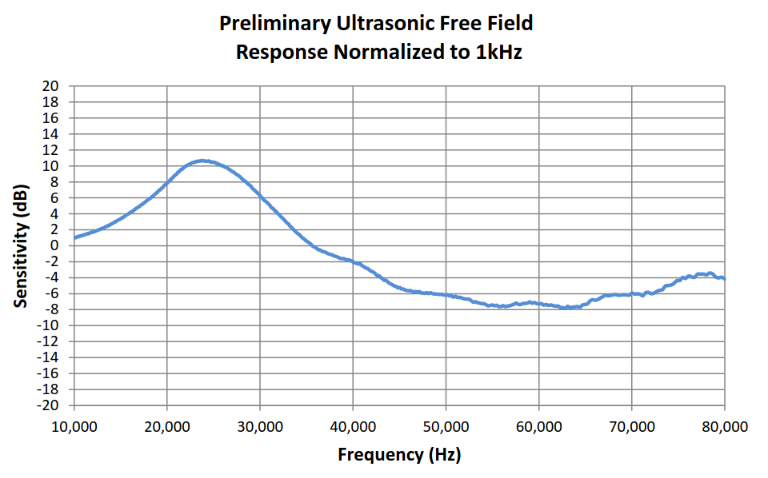
\includegraphics[width=0.8\textwidth]{mic_response.png}
    \caption{Pasmo przenoszenia mikrofonu SPU0410LR5H-QB}
    \label{fig:mic_response}
\end{figure}
\vspace{2cm}
\noindent

Następnym wymaganiem jest rozmiar. 
Wynika to z rodzaju pomiaru fali dźwiękowej, każdy z czujników wykrywa przecięcie sygnału z układem odniesienia. 
Odbiorniki nie powinny być oddalone od siebie bardziej niż połowa długości fali dźwiękowej. 
Czujniki mogłyby w przeciwnym razie wykrywać przecięcia z różnych okresów fali uniemożliwiając całkowicie obliczenie kąta padania. 
Długość fali jest zależna od częstotliwości sygnału oraz jego prędkości rozchodzenia się w danym medium. 
Wyznaczamy ją ze wzoru \ref{eq:wavelength} przy czym częstotliwość jest równa \unit[40]{kHz},
a prędkość rozchodzenia się dźwięku w powietrzu przy temperaturze 15 °C wynosi \unit[340,3]{m/s} \cite{sound_speed}.
Połowa długości fali to zatem \unit[4,25]{mm} i tej wartości nie powinna przekraczać odległość między odbiornikami.
Wszystkie czujniki tak małych rozmiarów są produkowane w technologii MEMS. 
\begin{equation}
\lambda = \frac{v}{f} = \frac{340,3\frac{m}{s}}{40kHz}=0,0085m = 8,5mm
\label{eq:wavelength}    
\end{equation}

\noindent
\vspace{2cm}

Kolejnym wymaganiem jest takie umieszczenie otworu ciśnieniowego w obudowie, by skierowany był on wewnątrz laminatu obwodu drukowanego. 
Taka konstrukcja jak na rysunku \ref{fig:mic} \todo{cite microphone datasheet}pozwala na stworzenie płaskiej powierzchni, tylko z otworami ciśnieniowymi czujników. 
Przekłada się to na mniejsze zakłócenia spowodowane odbiciami fali dźwiękowej od elementów elektronicznych.

\begin{figure}[ht!]
    \centering
    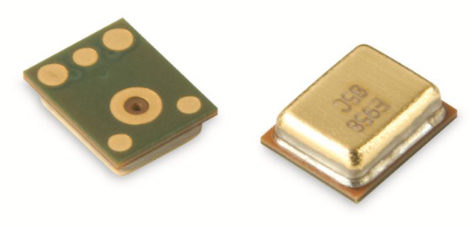
\includegraphics[width=0.8\textwidth]{mic.png}
    \caption{Mikrofon SPU0410LR5H-QB}
    \label{fig:mic}
\end{figure}
\noindent
Ostatecznym wymaganiem była dostępność i przystępność cenowa produktu. Ze względu na tak rygorystyczne oczekiwania wybór zawęził się zaledwie do kilku pozycji.
Jedną z nich był mikrofon SPU0410LR5H-QB marki Knowles\cite{knowles}, który w odpowiedniej ilości został dostarczony przez Promotora.
\vspace{2cm}



\section{Komercyjne rozwiązania}
Na rynku znajduje się bardzo dużo ultradźwiękowych czujników odległości, ale względnie niewiele firm oferuje sonary bez ruchomych elementów.
Czołowym producentem urządzeń w takiej technologii jest TOPOSENS ze swoim produktem o nazwie ECHO ONE\textregistered.
Rysunek \ref*{fig:echoone}, który jest zdjęciem marketingowym produktu, sugeruje, że posiada on ultradźwiękowy nadajnik oraz trzy odbiorniki we wzorze tworzącym kąt prosty.

\begin{figure}[ht!]
    \centering
    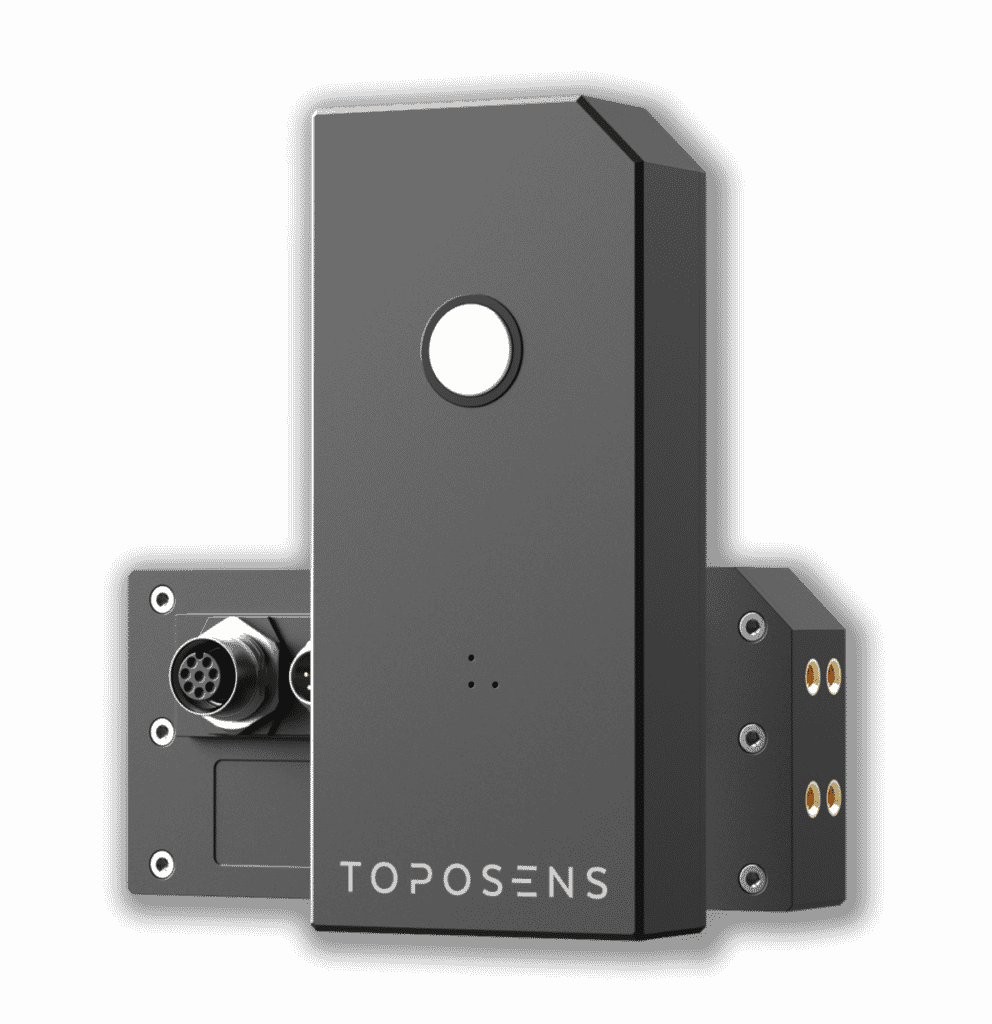
\includegraphics[width=0.5\textwidth]{ECHOONE.png}
    \caption{TOPOSENS ECHO ONE, źródło: https://toposens.com/}
    \label{fig:echoone}
\end{figure}

\chapter[Analiza problemu]{Analiza problemu}

\label{chapter:analiza_problemu}

% W tym rozdziale trzeba bardziej szczegółowo opisać jak chce Pan
% zrealizować cele sformułowane w rozdziale 2.
% Jakie będą konsekwencje i ewentualne wyzwania techniczne
% związane z przyjętą strategią. Jaka ogólnie ma być komunikacja
% z komputerem, tzn. czy to ma być tryb pytanie-odpowiedź, czy ciągłe
% przesyłanie danych. Czy być może jakiś tryb mieszany.
% Jaką chce Pan przyjąć formę przetwarzania danych i dlaczego. itd. itd.


\section{Plan urządzenia}

Założenia konstrukcyjne to przede wszystkim prostota budowy, modularność i skrócenie czasu realizacji. 
Płytka deweloperska wysyła określoną przez użytkownika liczbę przebiegów sygnału PWM (Pulse Width Modulation), 
następnie sygnał jest ten wzmacniany 
do poziomu aż \unit[80]{V} by uzyskać maksymalną wydajność i trafia na przetwornik piezoelektryczny który generuje falę ultradźwiękową.
Fala ta po odbiciu się od obiektu w polu wykrywania sonaru trafia z powrotem do urządzenia a konkretniej do mikrofonów MEMS umieszczonych na czole obudowy.
Sygnał z mikrofonów jest filtrowany by przepuścić tylko porządane przez nas częstotliwości bliskie czestotliwości nadajnika, 
oraz wzmacniany w celu lepszej interpretacji przez dalsze układy.

Po przefiltrowaniu, sygnał jest progowany. Mikrokontroler za pomocą przetwornika DAC ustala poziom napięcia, 
który wyznaczy granicę pomiędzy wysokim a niskim stanem logicznym. To rozróznienie jest nam potrzebne do pobudzenia cyfrowego wejścia licznika, 
zmienność tej wartości pozwala nam również na reagowanie tylko na sygnał o odpowiedniej amplitudzie by móc z powrotem obniżyć próg 
do miejsca przecięcia się sinusoidy z napięciem odniesienia, gdzie dokładność pomiaru jest największa.
Mikroprocesor dzięki wspomnianym wcześniej licznikom odmierza czas między zboczami rosnącymi zprogowanego już sygnału.
Wszystkie pomiary czasów przecieć z trzech odbiorników są wysyłane we wspólnej ramce danych do komputera gdzie za pomocą 
różnic w tych czasach wyznaczony zostanie dystans obiektu oraz jego odchylenie względem sonaru. Rys \ref{fig:uml}
\begin{figure}[ht!]
    \centering
    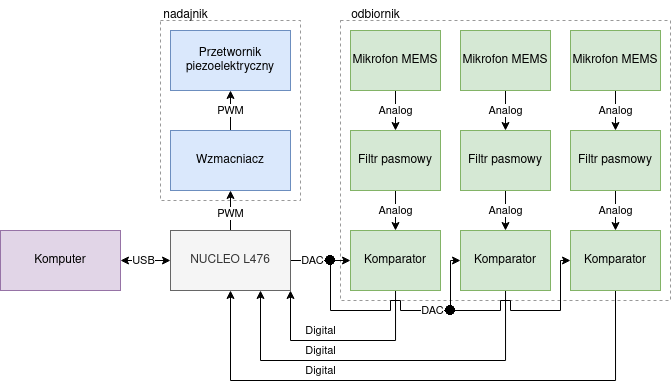
\includegraphics[width = 0.8\textwidth]{sonar_uml.png}
    \caption{Schemat blokowy urządzenia}
    \label{fig:uml}
\end{figure}



\section{Rozmieszczenie elementów nadawczych i odbiorczych}
Rozmieszczenie odbiorników jest kluczowym elementem pomiaru, to dzięki znajomości odległości mikrofonów i różnic w czasach 
dotarcia sygnału jesteśmy w stanie określić kąt pod którym fala dźwiękowa trafia do urządzenia. 
Do uzyskania pełnego zakresu w trzech osiach, wymagane są co najmniej trzy odbiorniki:
\begin{itemize}
    \item Mikrofon 0 -- mikrofon odniesienia, znajduje się on w centralnym punkcie, to według niego wyznacza będzie odległość od obiektu.
    \item Mikrofon X -- na podstawie pomiaru z tego mikrofonu wyznacza się kąt odchylenia w osi X 
    \item Mikrofon Y -- na podstawie pomiaru z tego mikrofonu wyznacza się kąt odchylenia w osi Y
\end{itemize}

\begin{figure}[ht!]
    \centering
    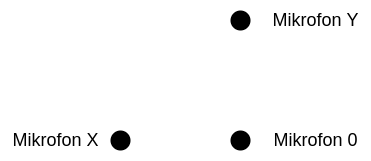
\includegraphics[width = 0.5\textwidth]{rozmieszczenie_mic.drawio.png}
    \caption{Rozmieszczenie mikrofonów}
    \label{fig:rozmieszczenie_mic}
\end{figure}

\section{Generowanie i odbieranie sygnału ultradźwiękowego}

\section{Komunikacja}
Komunikacja komputera typu PC z płytką deweloperską Nucleo na której bazowany jest projekt odbędzie się przy pomocy portu szeregowego. 
Każdy nowoczesny komputer posiada złącze USB, które miało niezwykły wpływ na standaryzacje interfejsów w urządzeniach użytkowych, 
większość płytek deweloperskich również posiada wbudowane gniazdo USB z portem szeregowym, dlatego też wybór tego rodzaju kompunikacji wydaję się wręcz oczywistą decyzją.
Tym samym złączem wgrywany jest również program do pamięci mikrokontrolera co jeszcze bardziej upraszcza stanowisko testowe.
Dane będą wysyłane w postaci tekstu w formie ,,pytanie-odpowiedź", zagwarantuje to większą elastyczność i możliwość zmiany parametrów urządzenia bez konieczności zmiany programu. 
W celu uruchomienia sekwencji wykrywania obiektu operator powinień wysłać komendę przykładowo o nazwie "START". 
Komenda taka posiadać będzie swoje ID w formie pojedynczej cyfry, pozwoli to zmniejszyć ilość znaków zamieszczanych w ramce danych. 
Komunikacja tekstowa przede wszystkim pozwala na weryfikacje danych przez standardowy terminal tekstowy. 
Ramka danych rozpocznie się znakiem ,,X", pomoże to programowi odfiltrować tylko dane przeznaczone dla niego. ,,X" został wybrany ze wględu na to, 
że znak ten na pewno nie będzie występował w treści wiadomości w żadnej postaci.
Wiadomość startu wraz z opcjonalnymi parametrami takimi jak ilość impulsów do wyemitowania czy próg czułości wykrywania sygnału wysłane są bajt po bajcie do urządzenia. 
Sonar rozpoznając znak początku ramki przechodzi dalej do odczytywania ID komendy oraz jej parametrów, po odebraniu całej wiadomości program zaczyna sekwencję pomiaru.
Następnie urządzenie wysyła do użytkownika odpowiedź, standardowo zaczyna znakiem rozpoznawczym a następnie zwraca numer ID komendy na którą ta wiadomość jest odpowiedzią,
status wykonania zadania, w formie kodów błędów, liczba wykrytych przecieć zer, czas kontrolny\todo{sprawdzić czy na pewno}, oraz wartości liczników z każdego ze składowych pomiaru.
Dane będą przetwarzane przez operacje na obiektach typu {\tt string}. Pozwoli to na wycięcie odpowiednich wartości ze scalonej ramki wysłanej jako jeden długi ciąg znaków.


% Lorem ipsum: \todo{jak dane są wyciagane z ramki, ogólny opis, port szeregowy, czemu tekstowo?}
% wybrano komunikacje tekstwoa co pozwalaa na zweryfikowanie danych poprzez zwykly teminal tekstowy nie powoduje obnizenia ofektywnosci kominikacji urzadzenia z komputerem 
% przyjeto komunikacja zapytanie odpowiedz, ze wzgledu na wieksza elastycznosc i mozliwosc zmiany ustawien sonaru 
% funkcje



\chapter[Specyfikacja realizacji sonaru ultradźwiękowego]{Specyfikacja realizacji sonaru ultradźwiękowego}

\label{chapter:specyfikacja}

Urządzenie, oprócz dostarczania swoich podstawowych funkcji niezbędnych do działania, 
może również zaoferować pewne udogodnienia w testowaniu oraz obsłudze przez użytkownika końcowego.
Takim udogodnieniem jest na pewno zmiana istotnych parametrów sonaru poprzez komunikację szeregową z urządzeniem.

Komendy, które przyjmuje urządzenie, to:
\begin{itemize}
    \item uruchomienie pomiaru -- rozpoczyna kompletną sekwencje pomiarową i zwraca wynik z powrotem do urządzenia;
    \item zmiana liczbę impulsów nadajnika -- za parametr przyjmuje wartości od 1 do 10 powtórzeń;
    \item zmiana wypełnienia impulsu -- wpływa na moc nadajnika, za parametr przyjmuje wartości (0-199), które odpowiadają największemu i najmniejszemu wypełnieniu;
    \item zmiana progu wykrywania sygnału  -- pozwala na regulację czułości odbiornika, za parametr przyjmuje 12-bitową wartość (0-4095) przetwornika DAC;
    \item zmiana czasu odstępu od zakończenia nadawania do rozpoczęcia odbierania, 
    za parametr przyjmuje czas wyrażony w taktach procesora o częstotliwości \unit[80]{MHz} w zakresie liczby 16-bitowej;  
    \item zmiana czasu końca pomiaru -- stanowi o tym, kiedy mikrokontroler powinien przerwać odbieranie sygnału, 
    za parametr przyjmuje czas wyrażony w taktach procesora o częstotliwości \unit[80]{MHz} w zakresie liczby 32-bitowej. 
\end{itemize}


% W tej części trzeba podać jakie będą udostępniane funkcjonalności,
% jak mają być realizowane pomiary, jakie polecenia będzie można
% przesyłać do urządzenia, przewidywane parametry, np.
% częstość powtórzeń pomiarów, zakres zmiany ilości sygnałów pobudzenia,
% zakres zmian wypełnienia impulsów itp.


\chapter[Projekt konstrukcji sonaru oraz protokoły komunikacji]{Projekt konstrukcji sonaru oraz protokoły komunikacji}

\label{konstrukcja}

Tutaj powinien być opis części mechanicznej, schematy elektroniczne,
opis protokołu komunikacji wraz z opisem implementacji (w protokole)
listy poleceń.
Opis funkcjonalności, które będą oferowane przez aplikację
oraz sposob przetwarzania danych pomiarowych i ich reprezentacji.

\section{Komunikacja}

\subsection{Wybór protokołu}

Wybrany został protokół UART, ze wględu na to, że płytka deweloperska STM32 NUCLEO-L476RG 
z której skorzystano w projekcie posiada wbudowany konwerter UART$\rightarrow$~USB, 
co pozwala na skomunikowanie mikrokontrolera z komputerem bez dodatkowego sprzętu.

\subsection{Komputer \textrightarrow{} sonar}
Użytkownik systemu może wysłać z komputera instrukcję do wywołania całej sekwencji działania urządzenia. 
Ramka danych zaczyna się znakiem specjalnym ułatwiającym rozpoznanie wiadomości, 
następnie musi zostać podany numer komendy informujący sonar jaką czynność powienien wykonać, 
parametry określające warunki tej czynności, a na koniec suma kontrolna wiadomości.

\begin{figure}[!ht] %data in
    \centering
    \begin{tikztimingtable}[timing/wscale=4]
        \tikzset{% Environment Config
            timing/dslope=0.1,
            timing/.style={x=5ex,y=2ex},
            x=5ex,
            timing/rowdist=3ex,
            timing/name/.style={font=\sffamily\scriptsize},
            timing/d/text/.style={font=\sffamily\tiny},
        }
        \textcolor{black}{Instruction} & [black]
            Z 1D{X}  1D{CMD\_ ID} 1D{PAR1} 1D{PAR2} 1D{PAR3}   1D{CRC}  \\ %
        \textcolor{black}{Bytes} & [black]
            Z 1D{1}  1D{1}        1D{1}    1D{1}    1D{4}      1D{4}    \\ %
        %
        % there must NOT be an uncommented line before \extracode!
        %
        \extracode
            \tablerules
        %%  \tablegrid
        
        \begin{pgfonlayer}{background}
            \begin{scope}[semitransparent ,semithick]
                %\vertlines[darkgray,dotted]{1.0,3.0,...,23.0}
                \vertlines[gray,dotted]{4.0,8.0,...,\twidth}
            \end{scope}
        \end{pgfonlayer}
        \end{tikztimingtable}
        \caption{Ramka danych przychodzących}
        \label{fig:datain}
    \end{figure}
    \todo{zrobić ładniejszą ramkę}

% \begin{figure}[!h]
%     \centering
%     \begin{tikztimingtable}[timing/wscale=4]
%         \tikzset{% Environment Config
%             timing/dslope=0.1,
%             timing/.style={x=5ex,y=2ex},
%             x=5ex,
%             timing/rowdist=3ex,
%             timing/name/.style={font=\sffamily\scriptsize},
%             timing/d/text/.style={font=\sffamily\tiny},
%         }
%         \busref*{FRAME}      & 2u 1d 2d 2u \\
%         \textcolor{black}{Instruction} & [black]
%             Z 1D{X}  1D{COM\_ID} 1D{CRC}    \\ %
%         \textcolor{black}{Bytes} & [black]
%             Z 1D{1}  1D{1}       1D{4}      \\ %
%         %
%         % there must NOT be an uncommented line before \extracode!
%         %
%         \extracode
%             \tablerules
%         %%  \tablegrid
        
%         \begin{pgfonlayer}{background}
%             \begin{scope}[semitransparent ,semithick]
%                 %\vertlines[darkgray,dotted]{1.0,3.0,...,23.0}
%                 \vertlines[gray,dotted]{4.0,8.0,...,\twidth}
%             \end{scope}
%         \end{pgfonlayer}
%         \end{tikztimingtable}
%     \end{figure}
    

\subsection{Sonar \textrightarrow{} komputer}

Sonar w odpowiedzi na instrukcję wysyła ramkę danych która również zaczyna się znakiem specjalnym, 
następnie podawany jest numer komendy na którą sonar odpowiada, status wykonania, dane pomiarowe oraz suma kontrolna.
\begin{figure}[!ht] %data out
\centering
\begin{tikztimingtable}[timing/wscale=4]
    \tikzset{% Environment Config
        timing/dslope=0.1,
        timing/.style={x=5ex,y=2ex},
        x=5ex,
        timing/rowdist=3ex,
        timing/name/.style={font=\sffamily\scriptsize},
        timing/d/text/.style={font=\sffamily\tiny},
    }
    \textcolor{black}{Instruction} & [black]
        Z 1D{X}  1D{ANS\_ID} 1D{STATUS} 1D{ZC\_NUM} 1D{TCL} 1D{D11} 1D{...} 1D{D33}  1D{CRC}  \\ %
    \textcolor{black}{Bytes} & [black]
        Z 1D{1}  1D{1}       1D{1}      1D{1}       1D{4}   1D{4}   1D{...} 1D{4}    1D{4}    \\ %
    %
    % there must NOT be an uncommented line before \extracode!
    %
    \extracode
        \tablerules
    %%  \tablegrid
    
    \begin{pgfonlayer}{background}
        \begin{scope}[semitransparent ,semithick]
            %\vertlines[darkgray,dotted]{1.0,3.0,...,23.0}
            \vertlines[gray,dotted]{4.0,8.0,...,\twidth}
        \end{scope}
    \end{pgfonlayer}
    \end{tikztimingtable}
    \caption{Ramka danych wychodzących}
    \label{fig:dataout}
\end{figure}
\todo{zrobić ładniejszą ramkę}


\section{Elektronika}
Projekt bazuje na autorskiej płytce z obwodem drukowanym, który został zaprojektowany przy pomocy 
otwartoźródłowego narzędzia do projektowania elektroniki ,,KiCad" \cite{kicad}.

\subsection{Zasilanie}
Całe urządzenie zasilane jest z portu USB komputera, które jednocześnie służy do komunikacji. 
Przewód jest podłączony bezpośrednio do płytki deweloperskiej Nucleo, 
a zaprojektowane na cele pracy dyplomowej PCB\footnote[1]{Printed Circuit Board ang. Płytka obwodu drukowanego}, 
jest podłączone do Nucleo w formie ,,shieldu"\todo{pokazać jak wygląda shield} poprzez listwy kołkowe. 
Mimo, że płytka deweloperska posiada wyprowadzenia zarówno 5V jak i 3.3V, które potrzebowałem, 
postanowiłem zaimplementować układ stabilizacji w celu lepszej izolacji zasilania układów analogowych od cyfrowych co powinno przełożyć się na mniejsze zakłócenia.
\begin{figure}[ht!]
    \centering
    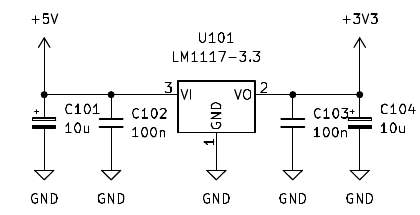
\includegraphics[width = 0.5\textwidth]{LDO.png}
    \caption{Stabilizator napięcia}
    \label{fig:ldo}
\end{figure}


\subsection{Część nadawcza}

\begin{figure}[ht!]
    \centering
    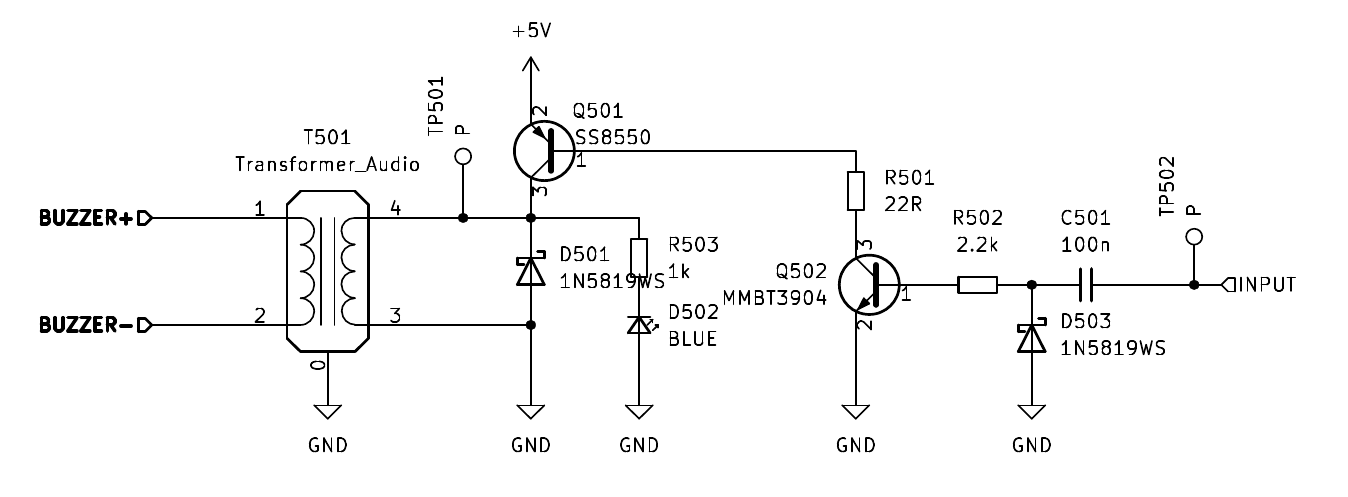
\includegraphics[width = \textwidth]{piezo.png}
    \caption{Wzmacniacz sygnału nadajnika piezoelektrycznego}
    \label{fig:piezo}
\end{figure}

\subsection{Część odbiorcza}
\begin{figure}[ht!]
    \centering
    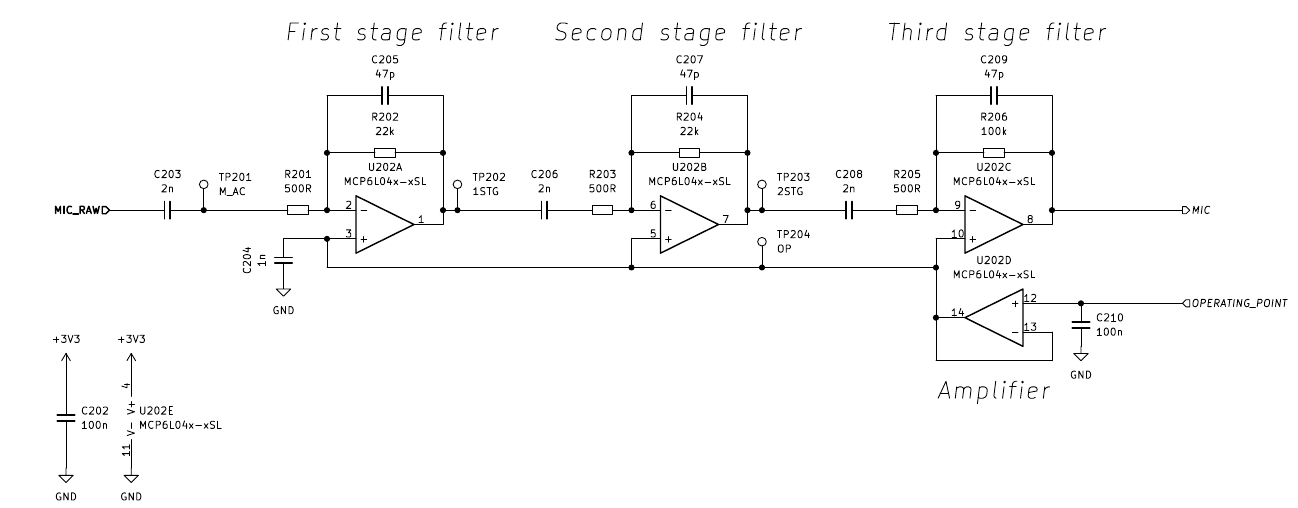
\includegraphics[width = \textwidth]{filter.png}
\end{figure}

\subsection{Symulacja części odbiorczej}

\chapter[Realizacja sonaru ultradźwiękowego]{Realizacja sonaru ultradźwiękowego}

\label{realizacja}

Opis wykonanego urządzenia, zdjęcia.
Przykłady realizacji komunikacji z urządzeniem.

\chapter[Testy i eksperymenty]{Testy i eksperymenty}

\label{chapter:testy}

Opis zrealizowanych eksperymentów, które demonstrują
najważniejsze cechy urządzenia i czujnika.

\section{Test przetwornika piezoelektrycznego}
Pierwszym testem był test przetwornika, który jest nadajnikiem sygnału. Zasilono go bezpośrednio z generatora wbudowanego w oscyloskop, 
parametry zadane to sygnał sinusoidalny o napięciu \unit[5]{V} \todo{\em...},,peak to peak" czyli wartości szczytowej.
Elementem odbiorczym był inny przetwornik piezoelektryczny służący tylko do testów, został on umieszczony w odległości \unit[10]{cm} od nadajnika. 
Jego częstotliwość rezonansowa również wynosiła \unit[40]{kHz}.
Po podłączeniu sondy oscyloskopu do odbiornika ukazał się bardzo wyraźny sygnał w kształcie sinusoidy ustawionej na nadajniku.
Dźwięki otoczenia miały bardzo znikomy wpływ na zakłócenia, stanowiąc niewielki procent amplitudy. 
Zmiana częstotliwości o chociażby \unit[1]{kHz} wiązała się kilkudziesięciokrotnym spadkiem mocy sygnału, co potwierdzało dane z noty katalogowej elementu piezoelektrycznego.
\begin{figure}[!ht]
    \centering
    \missingfigure{screen z oscylo z przebiegiem sygnału z piezo}
    \caption{Przebieg sygnału odebrany innym przetwornikiem piezoelektrycznym}
    \label{fig:oscylo_piezo}
\end{figure}

\section{Test wpływu odległości na sygnał}
Z identycznym stanowiskiem pomiarowym co sekcję wyżej sprawdzono wpływ odległości czujników na moc i przesuniecie fazy sygnału. 
\todo{zdjęcie z oscylo z przesuniętym sygnałem i kilka testów na różne odległości}

\begin{figure}[!ht]
    \centering
    \missingfigure{screen z oscylo z przebiegiem sygnału z piezo}
    \caption{Przebieg sygnału odebrany innym przetwornikiem piezoelektrycznym, wpływ na odległość}
    \label{fig:oscylo_piezo2}
\end{figure}

\section{Pierwsze uruchomienie}
PCB z przylutowanymi elementami zostało podłączone do zasilacza laboratoryjnego dostarczającego \unit[5]{V} i ograniczeniem prądowym ustawionym na \unit[100]{mA}. 
Pierwsze uruchomienie sterownika\todo{???} sonaru ujawniło drobny błąd projektowy, wszystkie diody elektroluminoescencyjne zostały przylutowane w złej polaryzacji.
Szybka zmiana ustawień diod i następne uruchomienie, nie pokazywało oznak większych błędów. Pobór prądu wyniósł\todo{podać ile prądu ciągnie}, a temperatura elementów na 
płytce nie odstawała od temperatury pokojowej.

\section{Uruchomienie i test wzmacniacza sygnału przetwornika piezoelektrycznego}

\begin{figure}[!ht]
    \centering
    \missingfigure{screen z oscylo z przebiegiem sygnału z piezo}
    \caption{Nadajnik sterowany przez wzmacniacz}
    \label{fig:oscylo_piezo3}
\end{figure}

\section{Test mikrofonów i filtrów}


\begin{figure}[!ht]
    \centering
    \missingfigure{screen z oscylo z przebiegiem sygnału z piezo}
    \caption{Przebieg sygnału odebrany innym przetwornikiem piezoelektrycznym}
    \label{fig:oscylo_piezo4}
\end{figure}


\chapter[Podsumowanie i wnioski]{Podsumowanie i wnioski}

\label{chapter:wnioski}

Ten rozdział pisze się jako przedostatni.
    Ostatnim jest "Wstęp"


\cleardoublepage
\phantomsection
\addcontentsline{toc}{chapter}{\bibname}
\bibliographystyle{alphapl}
\bibliography{sources/bibliografia}
\markboth{\bibname}{\bibname}   % to niestety nie działa by usunąć MakeUppercase z~nagłówków w~literaturze

%%spis tabel
%\cleardoublepage
%\phantomsection
%\listoftables
%\addcontentsline{toc}{chapter}{\listtablename}
%\markboth{\listtablename}{\listtablename}

%%spis rysunków
\cleardoublepage
\phantomsection
\addcontentsline{toc}{chapter}{\listfigurename}
\listoffigures
\markboth{\listfigurename}{\listfigurename}

\appendix
\chapter{Schematy i noty katalogowe}
\markboth{Schematy i noty katalogowe}{Schematy i noty katalogowe}

\begin{figure}
    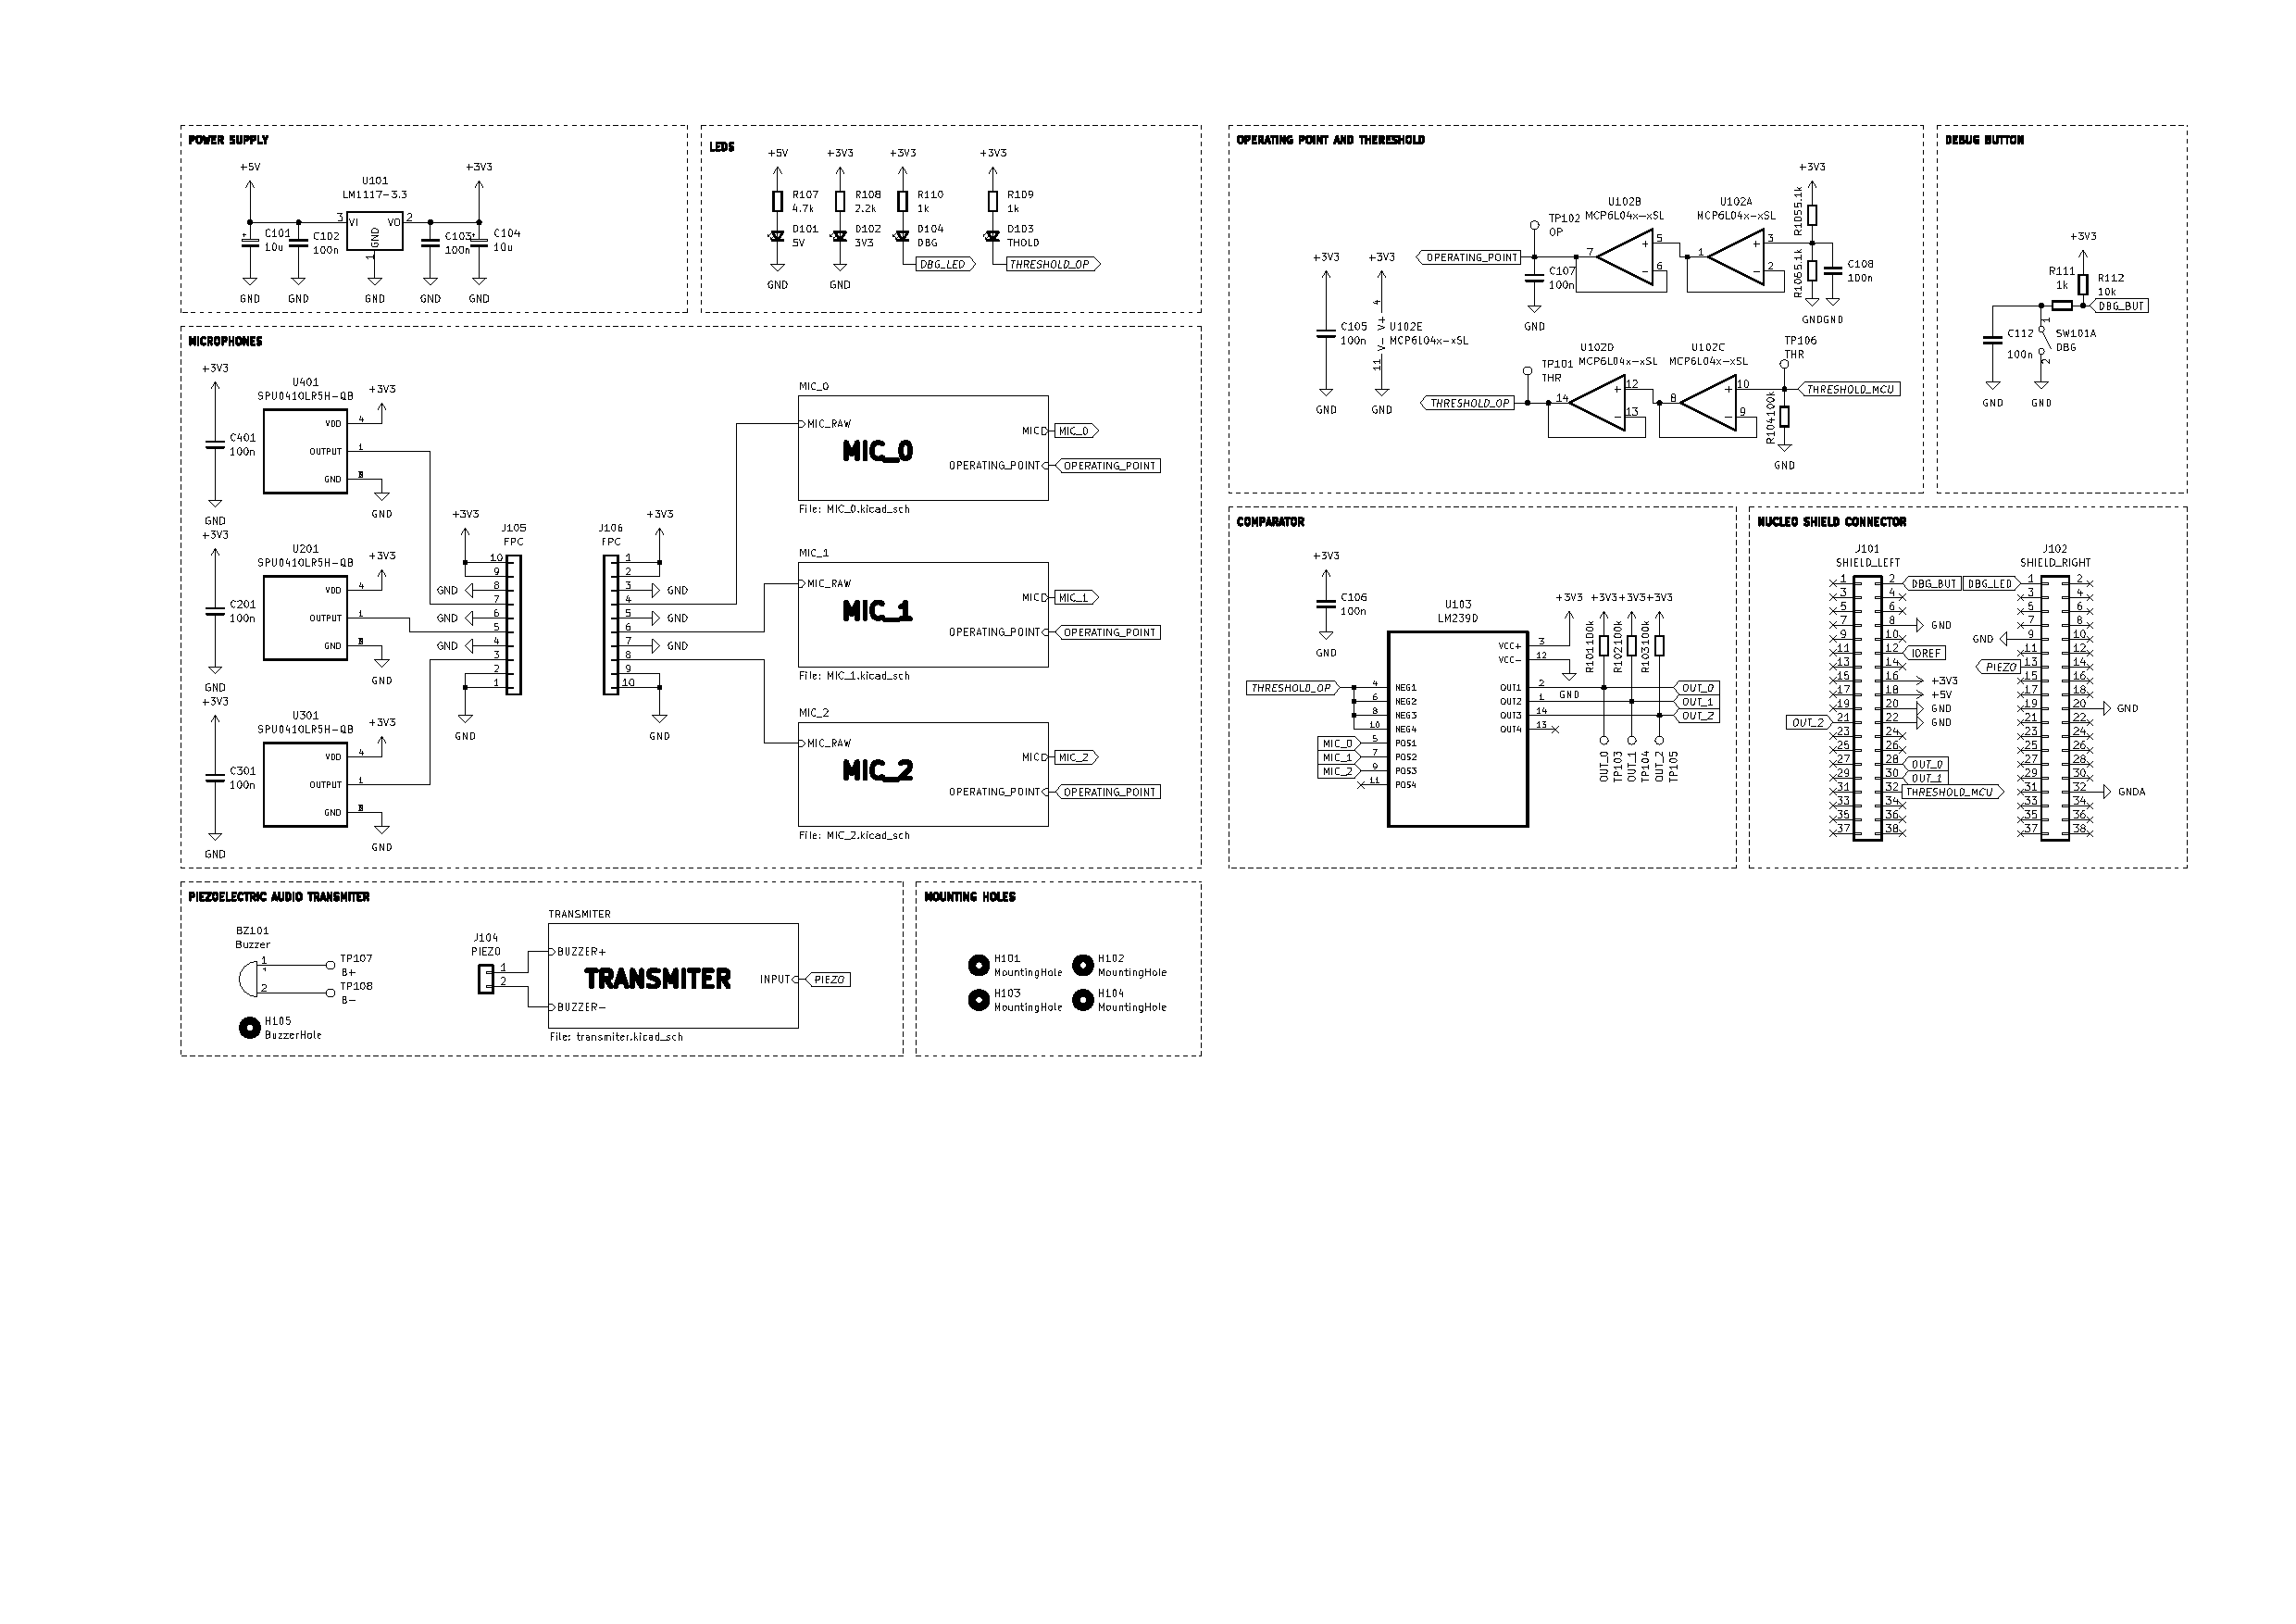
\includegraphics[width = \textwidth, trim=2cm 10cm 2cm 2cm, clip]{./figures/chapter_09/schemat_plytki.pdf}
\end{figure}

\begin{figure}
    \includegraphics[page = 2, width = \textwidth, trim=2cm 10cm 2cm 6cm, clip]{./figures/chapter_09/schemat_plytki.pdf}
\end{figure}

\begin{figure}
    \includegraphics[page = 5, width = \textwidth, trim=2cm 8cm 2cm 4cm, clip]{./figures/chapter_09/schemat_plytki.pdf}
\end{figure}

\begin{figure}
    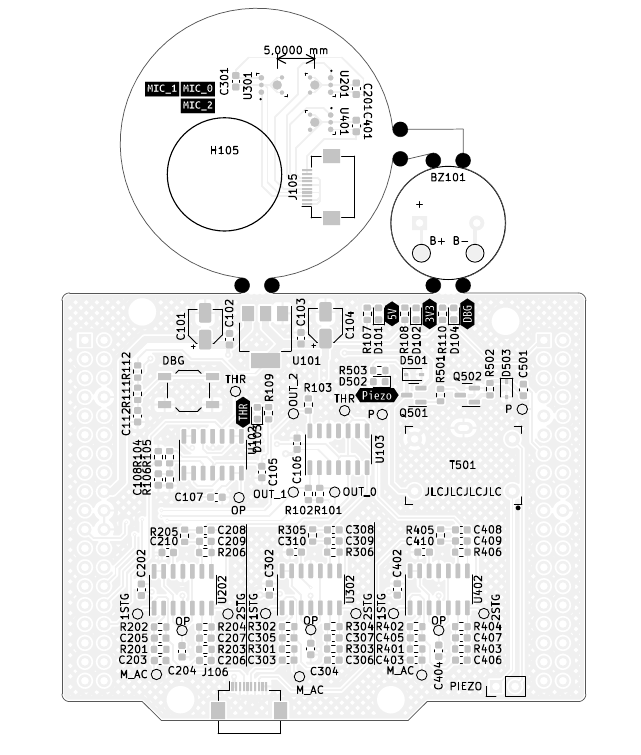
\includegraphics[width = \textwidth]{./figures/chapter_09/board_render.png}
\end{figure}

%% lista rzeczy do zrobienia
% \listoftodos

\end{document}
